\section{Introduction}
% TODO: rewrite the intro so that it will connect with chap1.

This chapter focuses on designs for high-speed ADCs in scaled CMOS technologies, which are required e.g. wireless ultra-wideband (UWB) communications.
Moreover, for wireless mobile devices, such ADCs should be power efficient to lessen the impact on battery life.

What are some common approaches to design high-speed and low-power ADCs?
The most common and popular approach is to time-interleave power-efficient SAR ADCs.
By heavily utilizing successive approximation circuitry, the ADC will become process scalable as well.
However, the downside of time-interleaving is that the core ADC area increases proportionally to the interleaved channels and will impact area cost. 
Moreover, inter-channel gain and timing mismatch calibrations increase complexity as well.
Flash ADCs are another option, which can realize high-speed with a minimum number of channels. 
However, Flash is notorious for its power-hungriness because a significant amount of redundant circuits must operate to obtain the conversion results.
To summarize, both ADC architectures have a design tradeoff between area and power and no optimum solution exist.

While ADCs must be designed to operate in the highest sampling frequency, such "highest speed" conditions are rarely used in real-life scenarios.
For example, in mobile communications, a single user will rarely use every channel (or frequency band) and the assigned frequency band will span reflecting the number of users in a particular environment.
Therefore, if there are lots of users in the environments, the assigned frequency band per user will be reduced (even with UWBs).
The available frequency band for a user maybe small as 20MHz or even up to 1 GHz if the environment is sparse.

\begin{figure}[!]
\centering
  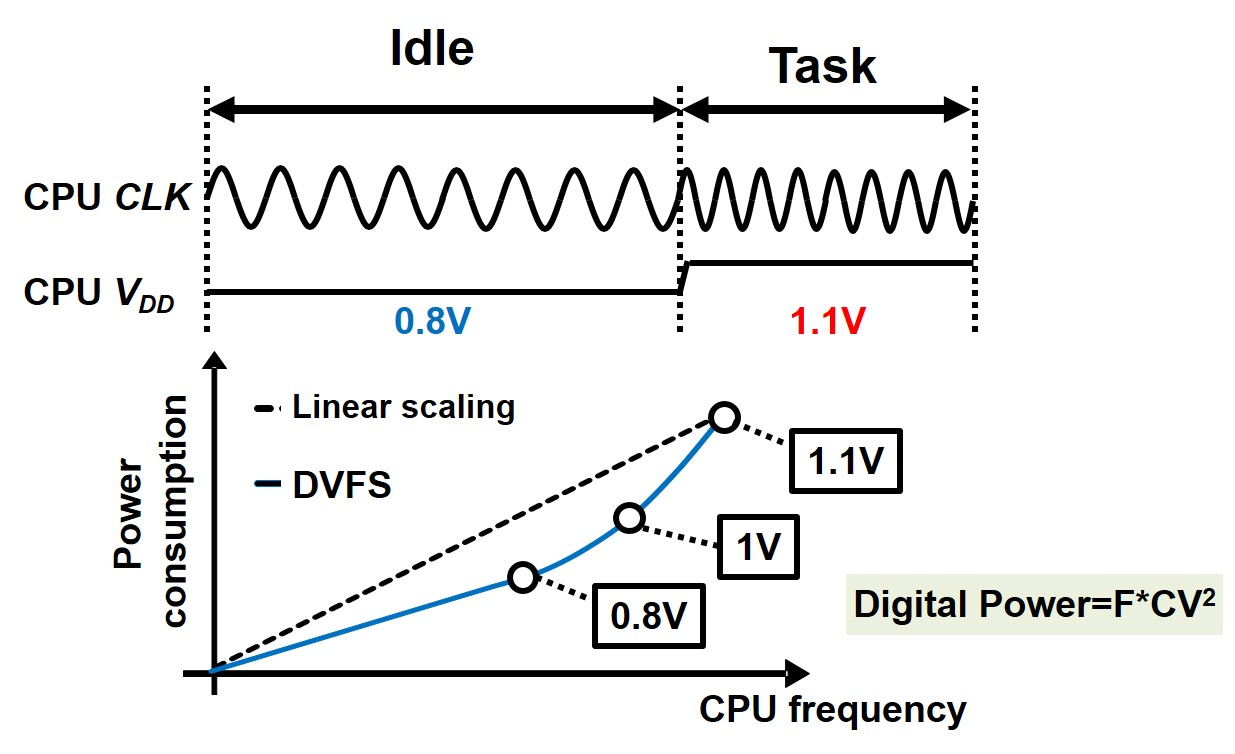
\includegraphics[width=0.9\textwidth]{figure/chap3/dvfs.jpg}
  \caption{Aggressive power scaling with DVFS, commonly utilized in CPUs.}
  \label{fig-dvfs}
\end{figure}

Our research question is: can we aggressively improve the high-speed ADC's frequency power scaling? Frequency power scaling is important, taking over the fact that the ADC sampling frequency spans widely during use.
Aggressive power scaling is commonly realized in CPUs as the dynamic voltage and frequency scaling (DVFS) technique (Fig.\ref{fig-dvfs}) \cite{DVFS}.
When the CPU is idle, the CPU lowers its operating frequency to save power. Simultaneously, it lowers its supply voltage to further reduce power (modern CPUs normally has a DC-DC converter per logic core). Since digital circuit power consumption is shown as:
\begin{equation}
    Power = C \times freq. \times V_{DD} ^2,
\end{equation}
lowering the supply voltage can aggressively reduce the power consumption.
Can we utilize the same technique in the ADC and simply lower its supply voltage when the required sampling frequency is low?
The answer might be negative because analog circuits have a much higher power supply sensitivity than digital; even lowering the power supply slightly will greatly reduce the sampling rate.
Thus the voltage-scalable frequency band will be very narrow and only a small benefit will be gained. 
Moreover, the overhead of having a respective DC-DC converter per ADC core may be too large; typical high-efficiency DC-DC converters are much larger than the ADC itself.

\begin{figure}[!]
\centering
  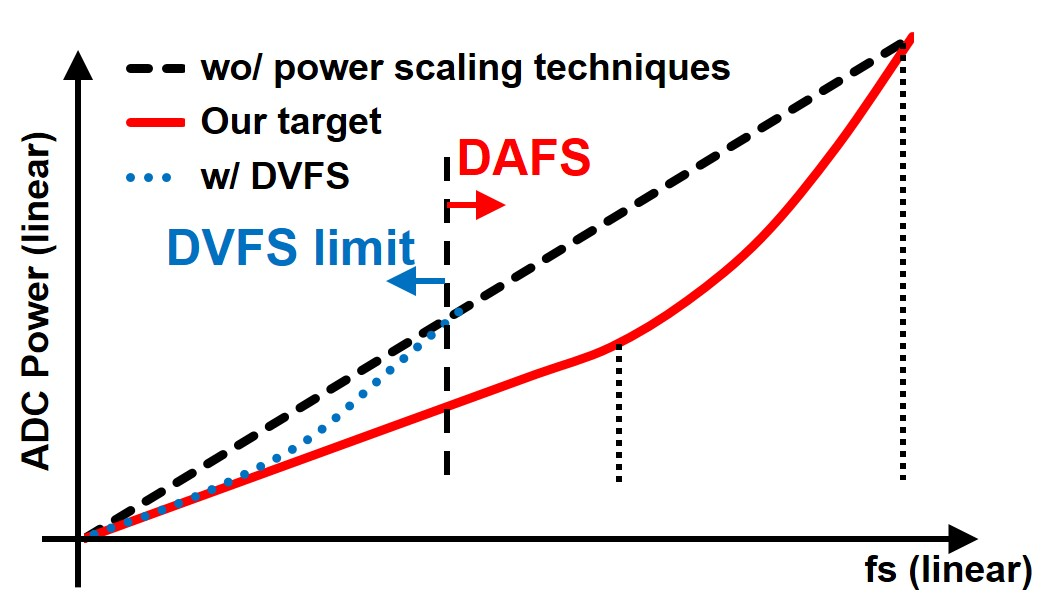
\includegraphics[width=0.9\textwidth]{figure/chap3/fig1.jpg}
  \caption{Dynamic power scaling of an ADC without any power scaling techniques, with DVFS, and with DAFS, respectively.}
  \label{fig-3-1}
\end{figure}

How can we achieve better frequency power scaling without tuning the supply voltage?
Our main idea is: configure between the successive approximation (SA) and flash ADC architectures dynamically, realizing a \textit{hybrid operation ADC}.
Such ADC will have the highest operating frequency of that of Flash and as the frequency slows down, the power consumption will reach that of the SA.
We will name such frequency scaling technique which dynamically switches architectures, the Dynamic Architecture and Frequency Scaling (DAFS) \cite{yoshioka2015dynamic}\cite{yoshiokaDAFS}. 

Fig.\ref{fig-3-1} compares the ADC power scaling with and without DAFS.
The Flash ADCs are reconfigurable so that it can be switched to operate as SA ADC as well.
By reconfiguring the ADC between SA and flash ADC every conversion cycle, the ADC achieves a maximum speed similar to Flash ADCs and a super-linear power scaling excelling that of the Flash, realizing a low-cost frequency power-scaling ADC.
DAFS not only improves the ADC power scaling but tracks the change in conversion delay caused by process, voltage, and temperature (PVT) variation as well.  As an example, if the ADC operates with slow corners, more flash operations will be inserted to reduce the excess-delay automatically. Since architecture configuring eases the speed variation effects, design margins when designing high-speed ADCs can be improved. 
To prove the DAFS effectiveness, a 7-bit subranging ADC was designed in 65nm CMOS and superlinear power scaling was observed in the range of 820 to 1220MS/s. 

This chapter is organized as follows: Section 3.2 describes the basic operation and analysis of DAFS with a simplified ADC. Section 3.3 presents a 7-bit subranging ADC that uses DAFS and describes its operation. The specific sub-ADC design is described as well. The experimental results and discussions are given in Section 3.4. 

\section{Dynamic Architecture and Frequency Scaling}

\subsection{Binary search (Successive approximation) and flash reconfigurable ADC}\label{BFADC}

\begin{figure}
\centering
  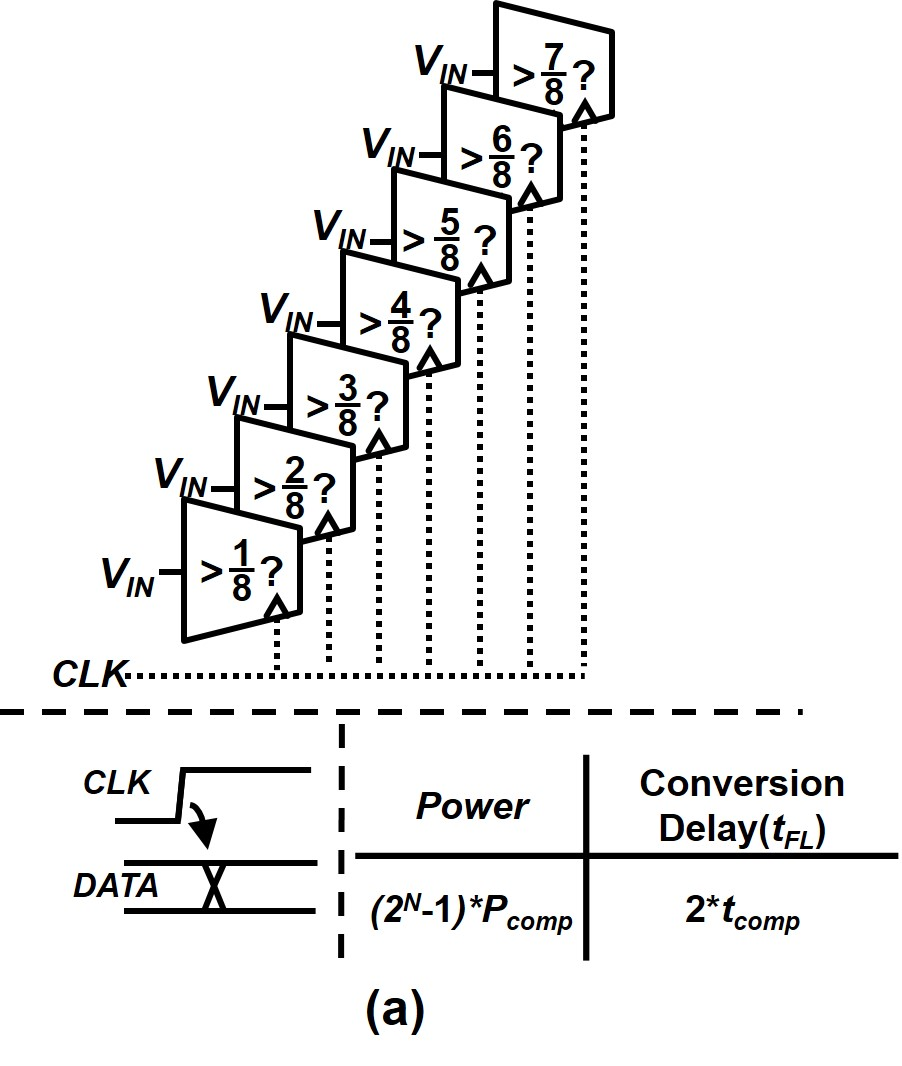
\includegraphics[width=0.6\textwidth]{figure/chap3/fig2a.jpg}
  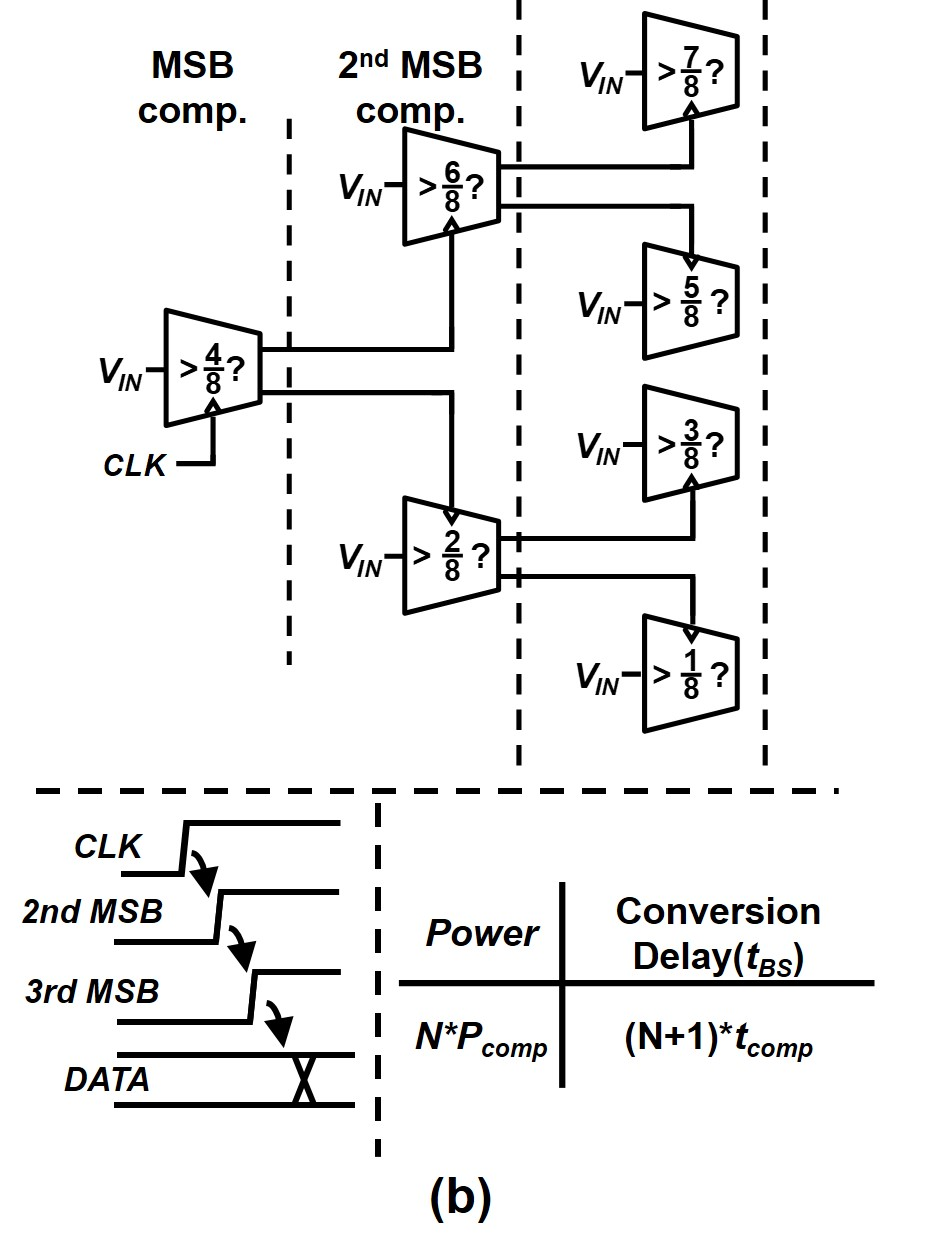
\includegraphics[width=0.6\textwidth]{figure/chap3/fig2b.jpg}
  \caption{ (a) Schematic of 3-bit flash ADC. (b) Schematic of 3-bit binary search ADC.}
  \label{fig-3-2}
\end{figure}

The proposed DAFS technique is based on two architectures, flash ADC and successive approximation (or binary searched) ADC \cite{van2008150}.
These two architectures are often used for high-speed ADCs with under 6-bit resolution and have a clear power and speed tradeoff. Firstly in Fig.\ref{fig-3-2} (a), a schematic diagram of a 3-bit flash ADC is shown. Seven comparators with different comparison thresholds ($>\frac{1}{8}$, $>\frac{2}{8}$, $>\frac{3}{8}$...) are used, and the flash ADC operates by simply activating all of the comparators at once. The flash ADC’s conversion delay ($t_{FL}$) is identical to single comparator delay ($t_{comp}$) plus the reset time of the comparator:

\begin{eqnarray}
  t_{FL} \simeq 2t_{comp}
\end{eqnarray}
Although this is the fastest ADC architecture, the flash ADC is notorious for its high power consumption. When the power of a single comparator is $P_{comp}$ and $N$ stands for the ADC resolution, the flash ADC power consumption ($P_{FL}$) can be expressed as
\begin{eqnarray}
  P_{FL} = (2^N - 1)P_{comp}
\end{eqnarray}
and $P_{FL}$ increases exponentially with $N$.

Secondly, a schematic of a 3-bit successive approximation (binary search) ADC is shown in Fig.\ref{fig-3-2} (b). 
While the "successive approximation" ADC mentioned here is fundamentally similar to "SAR" ADCs discussed in chapters 1 and 2, but its structure differs.
Since "successive approximation" ADCs are somewhat confusing, we will use the term "binary search ADCs" as used in the original paper.
SAR ADCs conduct a binary search by storing (or registering) the comparison results in the logic circuit and update the C-DAC reference voltage based on such data.
On the other hand, binary search ADCs change which comparator to activate based on the previous comparison results.

Like the flash architecture, the 3-bit binary search ADC uses seven comparators. When the CLK rise, only the MSB comparator is activated, which has a threshold of $\frac{4}{8}$. If the input is larger than $\frac{4}{8}$, the comparator with $\frac{6}{8}$ threshold is successively activated by the MSB comparator, based on a binary search algorithm. If the input is smaller than $\frac{4}{8}$, the comparator with $\frac{2}{8}$ threshold will be activated instead. Similarly, only one of the 3rd-bit comparators is activated, depending on the 2nd-bit comparator’s result. The conversion delay $t_{BS}$ including the comparator reset time will be:
\begin{eqnarray}
  t_{BS} \simeq (N+1)t_{comp}
\end{eqnarray}
While the maximum conversion speed is inversely proportional to $N$, the power efficiency is superior to that of the flash ADC.
Interestingly, unlike SAR ADCs the time for logic delays and C-DAC settling are not required in binary search ADCs, potentially achieving faster conversion speeds. However, the number of comparators increases exponentially with resolution and cannot be used for higher resolution.
\begin{eqnarray}
  P_{BS} = N \times P_{comp}
\end{eqnarray}
We can see that flash and binary search ADCs have a distinctive tradeoff between power and speed, and DAFS exploits this characteristic to achieve both low-power and high-speed operation by configuring the architecture operation ratio of these two architectures adaptively during the ADC conversion. 

\begin{figure}
\centering
  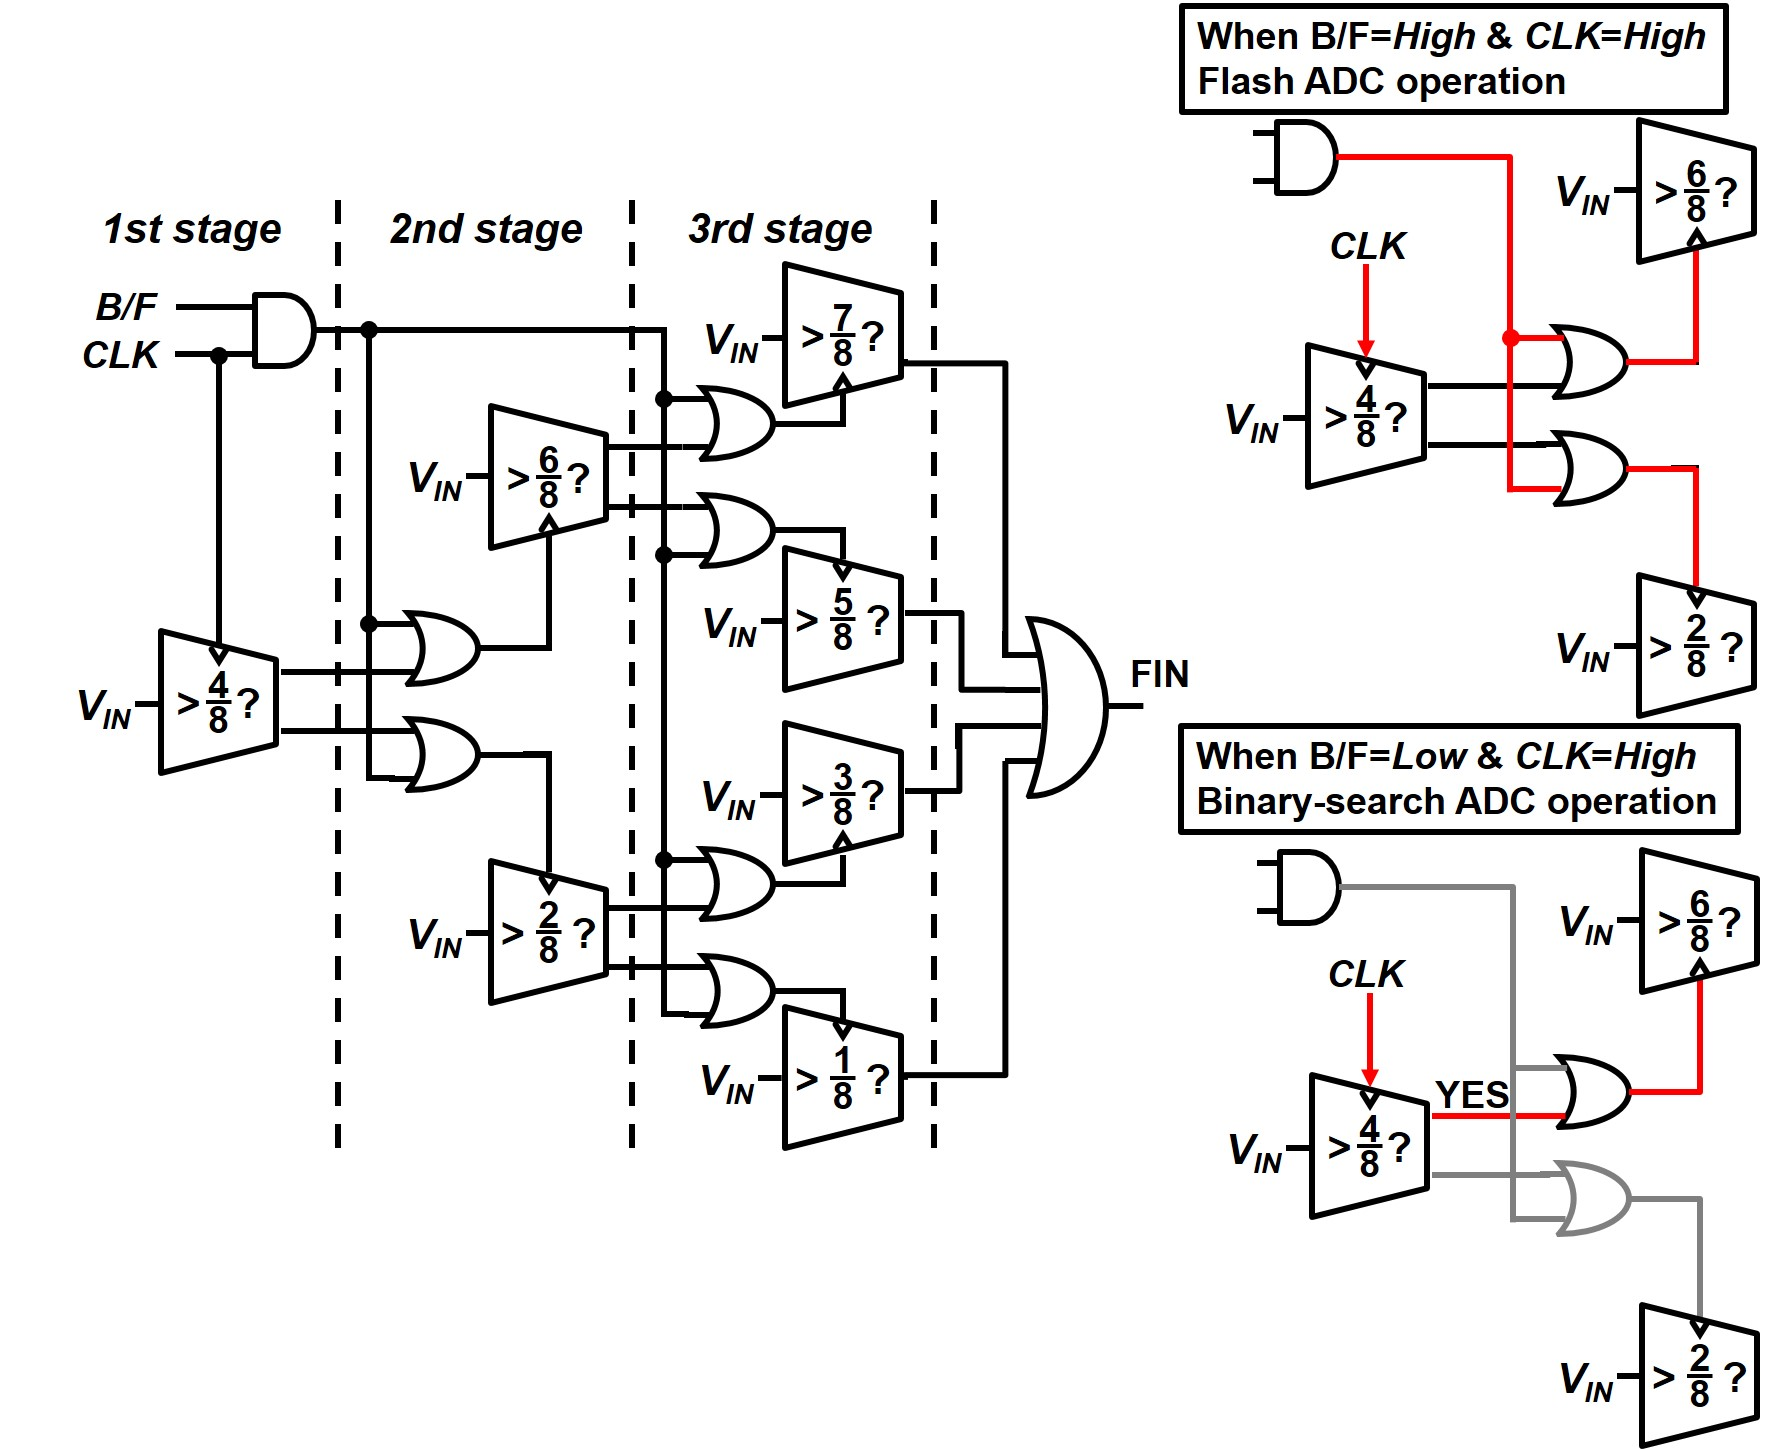
\includegraphics[width=1\textwidth]{figure/chap3/fig3.jpg}
  \caption{Schematic of the proposed binary search/flash reconfigurable ADC, realized by just adding OR cells to conventional Flash ADCs.}
  \label{fig-3-3}
\end{figure}

For the DAFS to work sufficiently, architecture reconfiguration between flash and binary search must be realized. 
Therefore, a binary search/flash reconfigurable ADC, which enables fast and simple reconfiguration, is proposed (Fig.\ref{fig-3-3}) by simply inserting OR cells between the comparator activation passes. 
The architecture configure signal (B/F) determines which ADC architecture to be used: when B/F is High, the ADC operates as a flash ADC; when B/F is Low, it operates as a binary search ADC.  
First, we will explain the ADC operation when signal B/F is $High$ and CLK rises. In such cases, the AND cell outputs $High$ to all of the OR cells which in turn output $High$ as well. Therefore, the OR cells activate all of the comparators simultaneously, which is equivalent to a Flash ADC operation. 

On the other hand, when B/F is $Low$, the output of AND will be $Low$ as well. For the OR cells to output $High$, the previous comparator must supply $High$, which is similar to a binary search ADC operation. The overheads of the reconfiguration are single AND and (2$N$-2) OR cells, which is remarkably small in terms of area and delay. However, the additional clock path delivering the architecture control signal to each comparator increases the ADC power by 5\%. 

\subsection{DAFS operation}

\begin{figure}
\centering
  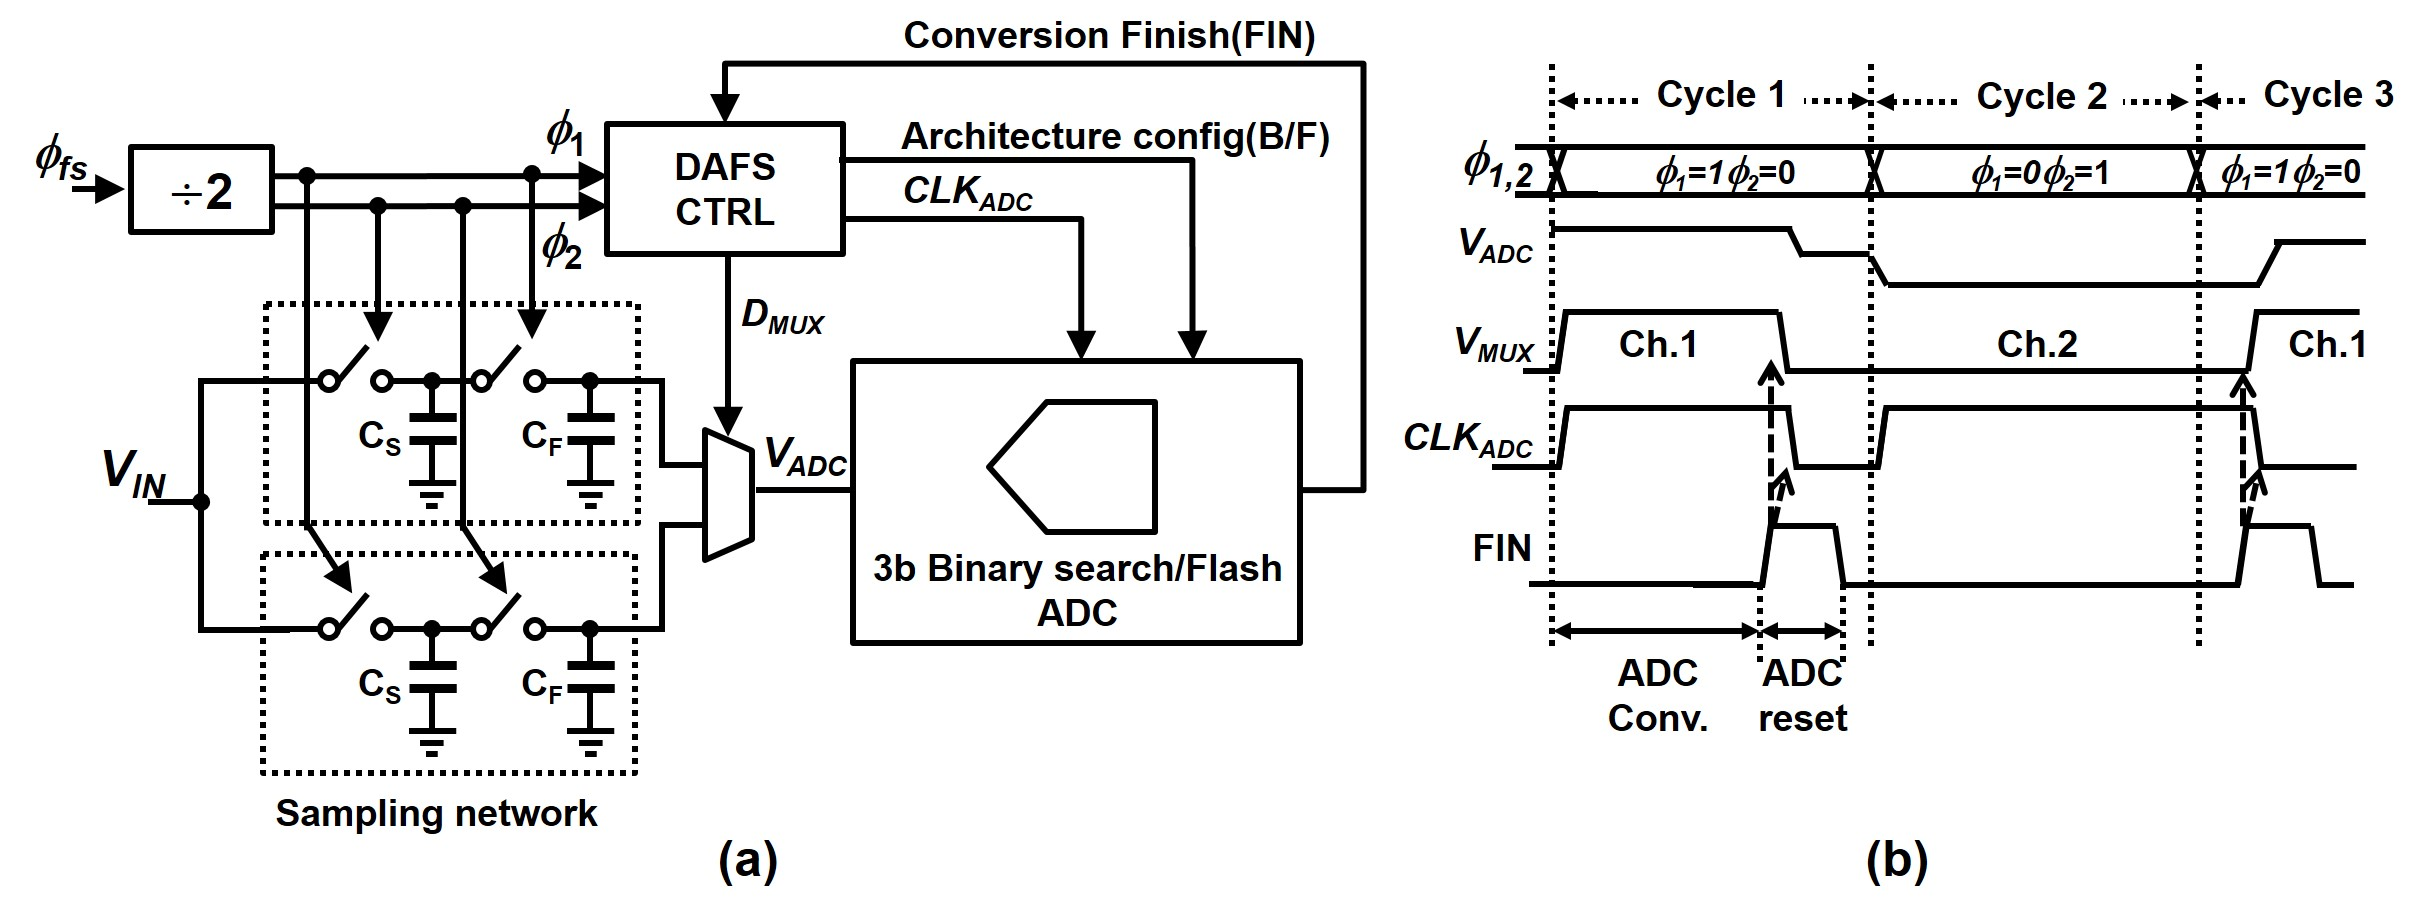
\includegraphics[width=1\textwidth]{figure/chap3/fig4.jpg}
  \caption{(a) Simplified test bench with a 3-bit ADC using DAFS. (b) Timing chart showing the basic operation of the ADC.}
  \label{fig-3-4}
\end{figure}

The basic concepts of the DAFS will be explained with a simple 3-bit ADC in Fig.\ref{fig-3-4} (a). As explained in \ref{BFADC}, the ADC is architecture reconfigurable and operates as a binary search ADC when the architecture configure signal (B/F) is Low and operates as a flash ADC when it is High. DAFS requires a 2-ch time-interleaved sample hold circuit (S/H), which makes the sampling network more complex than that of typical ADCs. As shown in the schematic of Fig.\ref{fig-3-4} (a), the ADC sampling network consists of 2-ch time-interleaved S/Hs and a MUX switches the input given to the ADC ($V_{ADC}$).

The basic timing chart is shown in Fig.\ref{fig-3-4} (b), and when CLKADC rises at the start of cycle 1, the ADC starts the conversion. As soon as the ADC finishes the conversion, the conversion finish signal (FIN) rises. FIN is fed to the control circuit (DAFS CTRL) to set down CLKADC and toggle DMUX to switch the input channel used in the next cycle. These actions are taken during the ADC conversion phase. In the subsequent ADC reset phase, as soon as CLKADC falls, the comparator outputs become reset and set down FIN. At this point, ADC is ready for the next conversion. 

\begin{figure}
\centering
  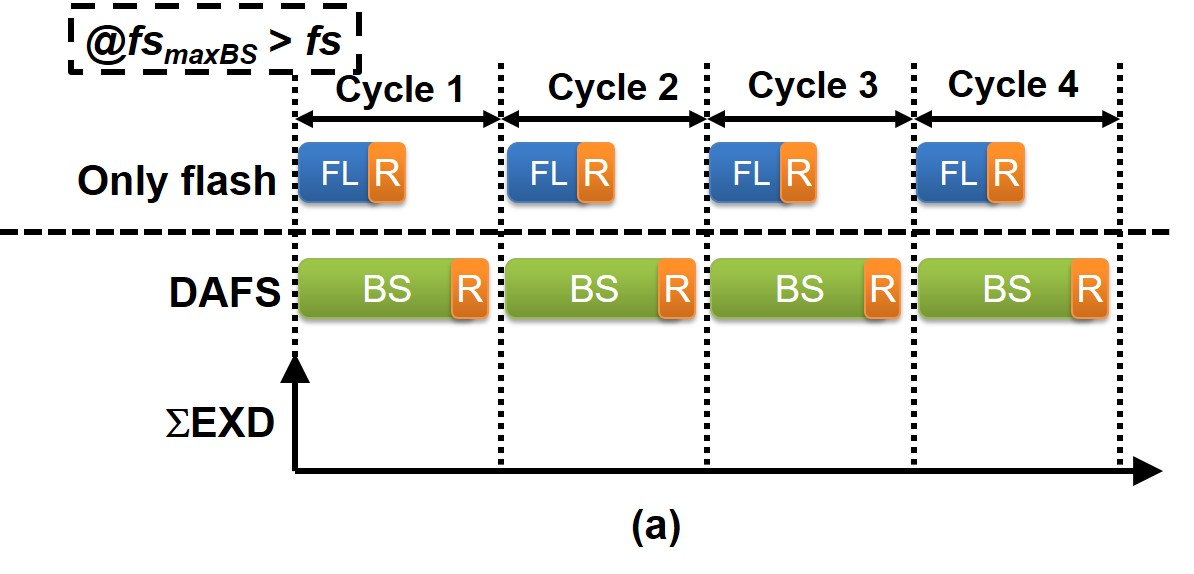
\includegraphics[width=0.8\textwidth]{figure/chap3/fig5a.jpg}
  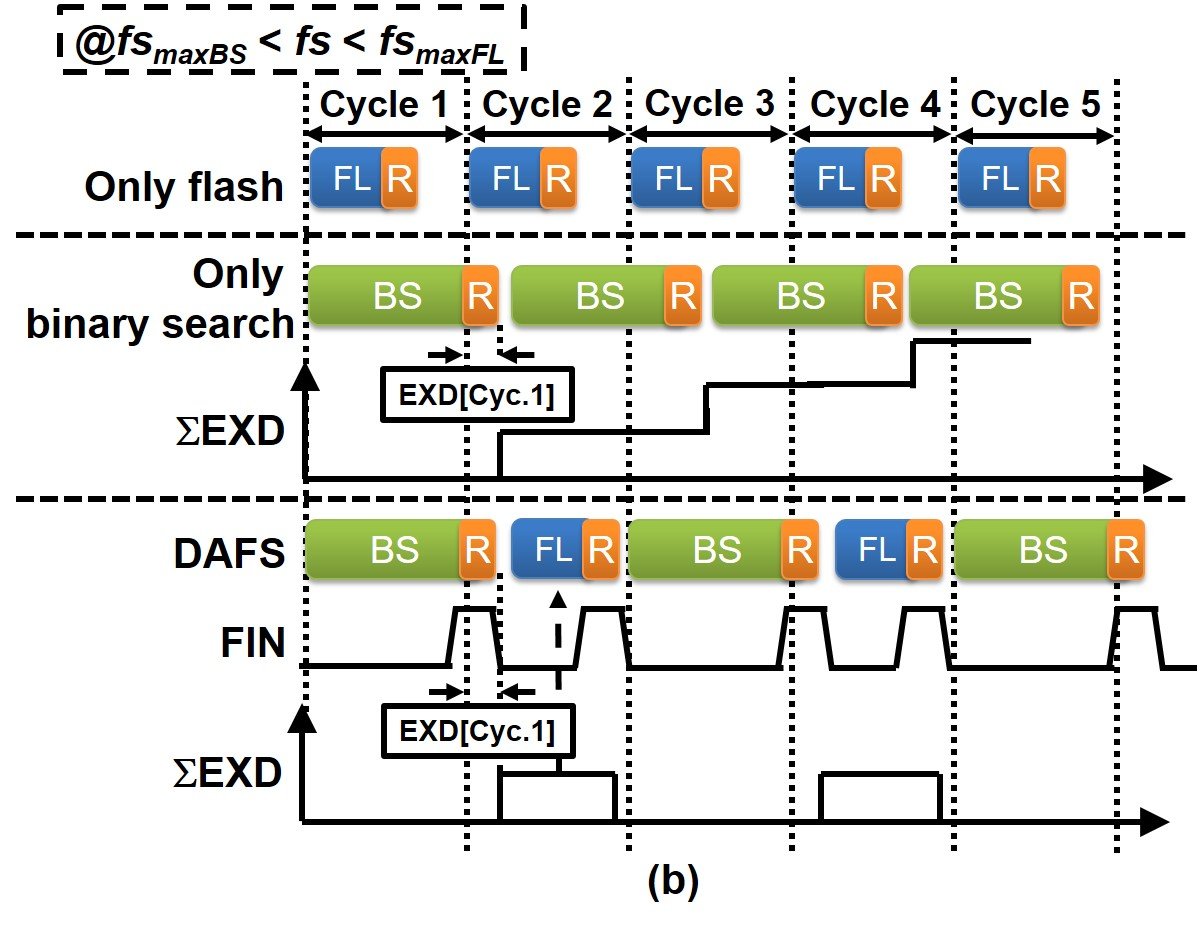
\includegraphics[width=0.8\textwidth]{figure/chap3/fig5b.jpg}
  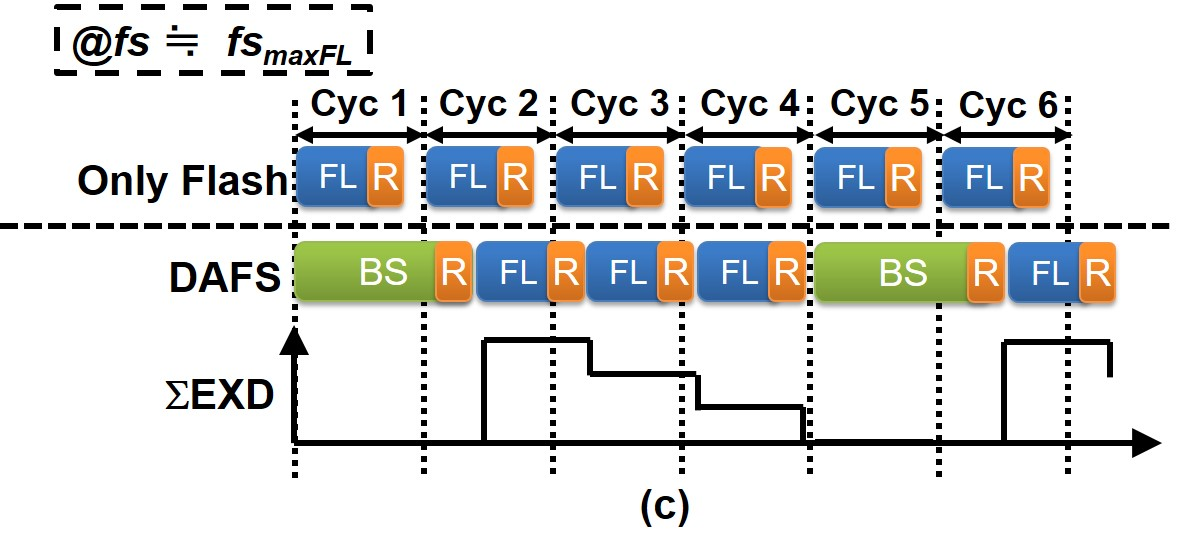
\includegraphics[width=0.8\textwidth]{figure/chap3/fig5c.jpg}
  \caption{(a) DAFS operation at $fs_{maxBS} > fs$. (b) DAFS operation at
$fs_{maxBS} < fs < fs_{maxFL}$. (c) DAFS operation at $fs \simeq fs_{maxFL}$.}
  \label{fig-3-5}
\end{figure}

Fig.\ref{fig-3-5} shows the ADC operation operated at several frequencies: $fs_{maxBS} > fs$, $fs_{maxBS} < fs < fs_{maxFL}$ and $fs \simeq fs_{maxFL}$. $fs_{maxBS}$ and $fs_{maxFL}$ is the maximum operation frequency for binary search and flash conversions, respectively. To start with, let us consider the DAFS ADC operation when $fs_{maxBS} > fs$ (Fig.\ref{fig-3-5} (a)) and for comparison, ADC operation with only flash is plotted as well. Since the flash conversion time ($t_{FL}$) is much shorter than the cycle ($\frac{1}{fs} = t_{cyc}$), the conversion is completed with a large margin. Conversely, the ADC is idle for over half of the given time $t_{cyc}$. The ADC reset time is indicated as $R$ in the figure. When DAFS is used, the ADC operates as binary search to reduce the power and since $fs_{maxBS} > fs$, the binary search conversion time ($t_{BS}$) is still shorter than $t_{cyc}$ and the conversion can be completed without any architecture configurations. 

Next, let us examine the ADC operation when $fs_{maxBS} < fs < fs_{maxFL}$ (Fig.\ref{fig-3-5} (b)).  Since $fs$ is still below $fs_{maxFL}$, flash conversion is completed with a margin. On the other hand, $fs$ is now higher than $fs_{maxBS}$, meaning that $t_{BS} > t_{cyc}$. The ADC operation with only binary search is also shown for comparison, and in which the binary search conversion does not finish within cycle 1 and prolonged into cycle 2. We can calculate the excess-delay (EXD) generated in cycle 1 as:
\begin{eqnarray}
  EXD[Cyc.1] = t_{BS} - t_{FL}
  \label{EXD}
\end{eqnarray}

EXD will occur every cycle and \eqref{EXD} will accumulate, meaning that the conversion will be corrupted once EXD occurs. However, by configuring the architecture to flash, the EXD can be canceled. The operation with DAFS is plotted, in which the DAFS CTRL circuit monitors if EXD is positive or not. Since a positive amount of EXD is detected at the beginning of cycle 2, B/F is turned to High and the ADC is configured to operate as a flash ADC in cycle 2. Intriguingly, $t_{FL} < t_{cyc}$ and the EXD of cycle 2 can be expressed as:
\begin{eqnarray}
  EXD[Cyc.2] = t_{FL} - t_{CYC} < 0
  \label{EXD2}
\end{eqnarray}
which is a negative value. Therefore, the total accumulated EXD ($\sigma$EXD) of these two cycles will be,
\begin{eqnarray}
  EXD[Cyc.1] + EXD[Cyc.2] = (t_{BS} - t_{CYC}) + (t_{FL} - t_{CYC}) < 0
  \label{EXD3}
\end{eqnarray}
Equation \eqref{EXD3} shows that by using the flash operation, the ADC succeeds in cancelling EXD produced in cycle 1. The A/D conversion can be continued while consuming significantly less power than ADCs conducting only flash operations.

Lastly, let us examine the operation when $fs \simeq fs_{maxFL}$  (Fig.\ref{fig-3-5} (c)). Here as well, the binary search operation in cycle 1 produces a large amount of EXD and hence, the ADC is configured to flash in cycle 2. However, as $fs$ rises the EXD canceling effect lessens.
\begin{eqnarray}
  EXD[Cyc.1] + EXD[Cyc.2] = (t_{BS} - t_{CYC}) + (t_{FL} - t_{CYC}) > 0
  \label{EXD5}
\end{eqnarray}
Therefore, not all of the EXD that arose at cycle 1 can be canceled at once, and the conversion is prolonged into cycle 3. Similarly, the DAFS CTRL circuit judges that EXD is still positive and the ADC operates as a flash at cycle 3 as well. The flash operation continues until EXD is completely canceled:
\begin{eqnarray}
\begin{split}
  EXD[Cyc.1] + EXD[Cyc.2] + EXD[Cyc.3] + EXD[Cyc.4] \\
  = (t_{BS} - t_{CYC}) + 3(t_{FL} - t_{CYC}) < 0
  \label{EXD4}
  \end{split}
\end{eqnarray}
In Fig.\ref{fig-3-5} (c), three times of flash operation is used to cancel the EXD produced by a single binary search operation. 

\subsection{Analysis of DAFS}
The above study for different \textit{fs} ranges makes mainly four points. (a) When \textit{fs} is higher than $fs{}_{maxBS}$, the flash operation begins to be inserted. (b) By conducting flash operations, excess-delay produced by binary search operation can be canceled. (c) The flash operation continues until the excess-delay is completely canceled. (d) The occurrence of the flash operation is proportional to \textit{fs}. 

This section further analyzes the ADC in terms of its response to PVT variations and power consumption. Firstly, let us define the binary search versus flash ratio (BF ratio) to signify how much flash operation is used during conversion at a specific \textit{fs}.
\begin{eqnarray}
  \mathrm{BF\ ratio=\ }\frac{Num.\ of\ Flash\ conv.}{Num.\ of\ BS\ conv.\ +Num.\ of\ Flash\ conv.} 
\end{eqnarray}

For example, the BF ratios of the operations shown in Fig.\ref{fig-3-5} are 0, 0.5 and 0.75. Next, let us estimate the BF ratio for a given \textit{fs}. When $fs{}_{maxBS}$ $\mathrm{>}$ \textit{fs}, the ADC operation is fully a binary search and BF ratio will always be 0. However, when \textit{fs}$\mathrm{>}$fs${}_{maxBS}$, there is a positive amount of EXD and flash operation will be used. The BF ratio, in this case, is determined from the number of flash conversions required to cancel EXD produced by a single binary search operation. Namely,

\begin{eqnarray}
  \mathrm{BF\ ratio=}\frac{(t_{BS}-t_{CYC})/(t_{CYC}-t_{FL})}{1+(t_{BS}-t_{CYC})/(t_{CYC}-t_{FL})}\mathrm{=}\frac{t_{BS}-t_{CYC}}{t_{BS}-t_{FL}}
  \label{eq3.11}
\end{eqnarray}

If we suppose that \textit{t${}_{BS}$} and \textit{t${}_{FL}$} are insensitive to the input signal, the BF ratio for specific \textit{fs} can be estimated. Moreover, if we substitute $\frac{1}{fs}=t_{cyc}$, we can express (\ref{eq3.11}) with frequency as below.
\begin{eqnarray}
  \mathrm{BF\ ratio=}\frac{{fs}_{maxFL}}{fs}\left(\frac{fs-{fs}_{maxBS}}{{fs}_{maxFL}\mathrm{-}{fs}_{maxBS}}\right)
  \label{eq3.12}
\end{eqnarray}

Two interesting characteristics of DAFS can be studied with the help of equations \eqref{eq3.11} and \eqref{eq3.12}: PVT drift tracking and power consumption. To start with, let us examine how the BF ratio changes with PVT drift. Here, we will assume that a PVT drift will slow down the transistor (i.e. higher temperature, slow corners) and increase \textit{t${}_{BS}$} and \textit{t${}_{FL}$}. As a result, the binary search operation produces more EXD, and the amount of EXD canceled by flash operation decreases as well. Thereupon, the number of flash operations increases as well as the BF ratio. On the other hand, with faster transistors, the BF ratio decreases because less EXD is produced and more EXD can be canceled with flash.  Normally when designing high-speed ADCs, we must put a lot of design margins into the circuit to meet the target \textit{fs} even in the slowest corner condition, and this can lead to a large power overhead. With DAFS, this design margin can be significantly relaxed. 

\begin{figure}
\centering
  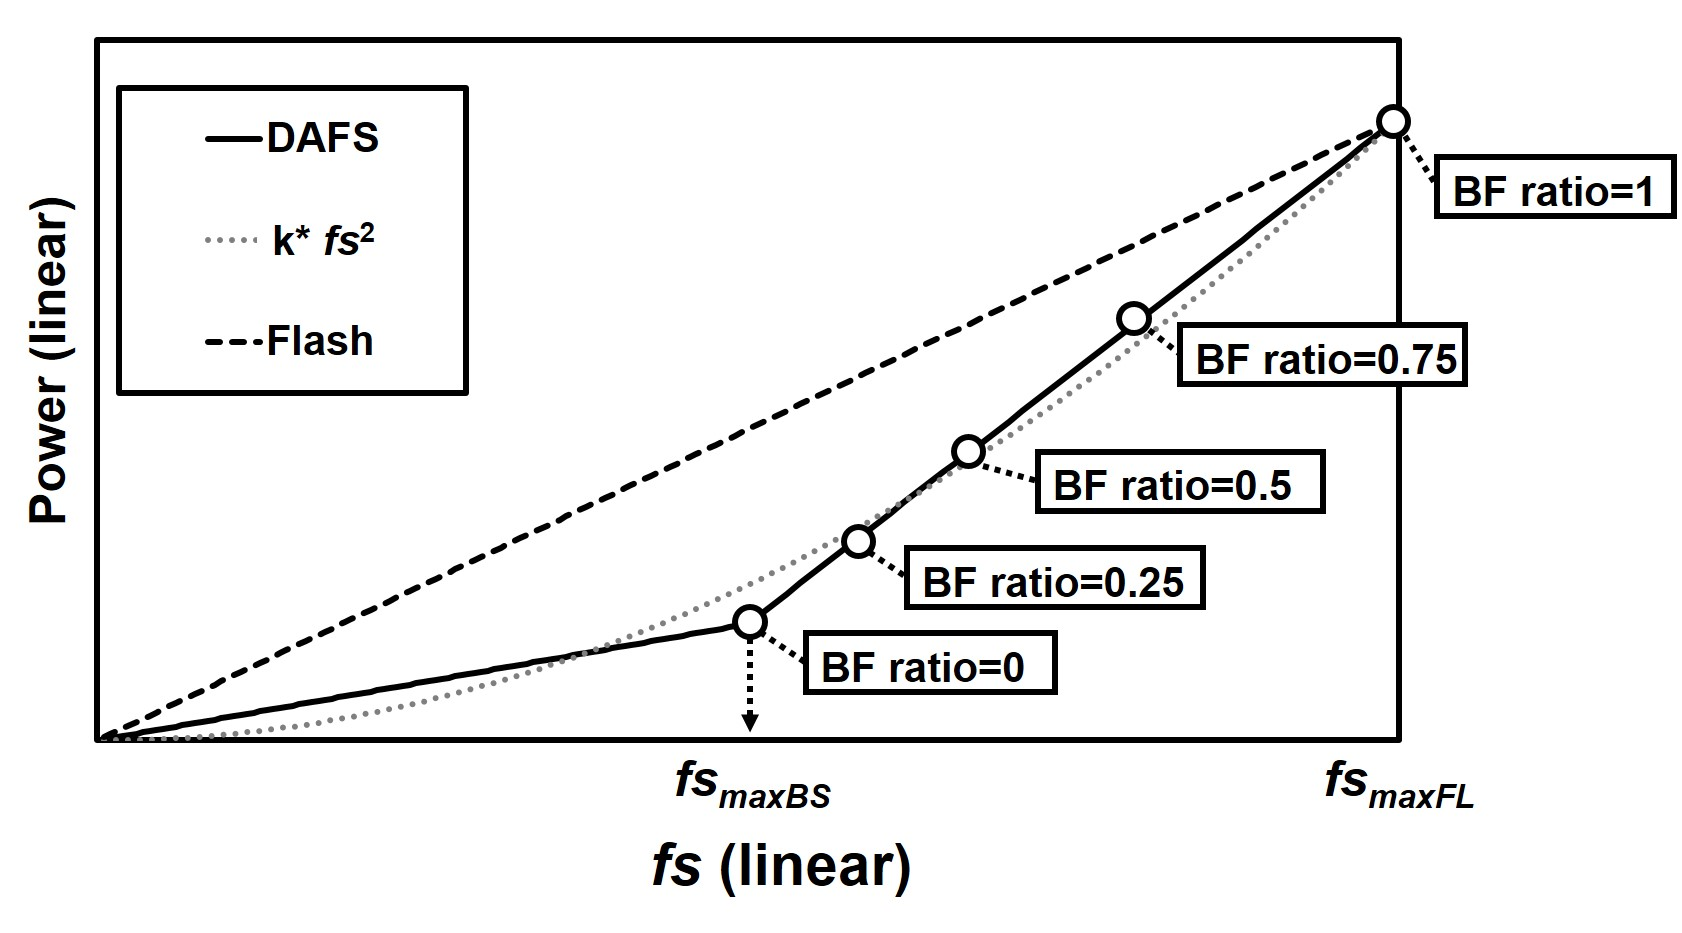
\includegraphics[width=0.8\textwidth]{figure/chap3/fig6.jpg}
  \caption{Dynamic power scaling of an ADC operating only with flash and with DAFS, respectively}
  \label{fig-3-6}
\end{figure}

Second, the ADC power consumption (\textit{P${}_{ADC}$}) is estimated from the BF ratio; this is useful when designing and analyzing DAFS ADCs. Our goal is to express \textit{P${}_{ADC\ }$}with \textit{fs}, which represents the ADC power scaling. While deriving the exact power scaling is cumbersome, we can simply understand DAFS power scaling as a linear scaling having two regions.

\begin{align*} 
 P_{ADC}=fs\times {P_{BS}}[fs <= {fs}_{maxBS}] \\
 P_{ADC}=fs\times \left(P_{BS}+\alpha \right) [fs>{fs}_{maxBS}]
 \label{eq3.16}
\end{align*}
As $fs$ excels $fs_{maxBS}$ and Flash operation begins to be inserted, the power scaling function changes to that of the latter.

Here, $\alpha$ is a constant expressing the additionally-inserted Flash operations. We can see that the DAFS ADC power scaling is a linear power scaling, in which its slope increases when the \textit{fs} exceeds $fs{}_{maxBS}$. The DAFS power scaling for an ADC resolution of 3-bit has been plotted in Fig.\ref{fig-3-6}, with a power scaling of the flash ADC for comparison. By dynamic architecture configuration, superlinear power scaling can be obtained. The entire power scaling curb of the DAFS can be fit to a quadrature scaling of k*\textit{fs}${}^{2}$, where k is a constant which meets
\begin{eqnarray}
k=\frac{{{P}}_{{FL}}}{{fs}_{maxFL}},
\end{eqnarray}
thus we can call this power scaling "super-linear".

In ADCs using DAFS, the EXD produced by a binary search can be canceled by the flash operation as long as its duration is within a cycle. Conversely, DAFS can only be used when ${\mathrm{t}}_{BS}<2t_{CYC}$. If the ADC does not meet this requirement and conducts a binary search in cycle \textit{N}, it cannot do any conversion at cycle \textit{N}+1 and there will be a loss of data. Furthermore, when the resolution of the binary search/flash configurable ADC is increased, \textit{$t_{BS}$} will become larger as in (3.5) and DAFS cannot be used up to \textit{$fs_{maxBS}$}. Hence, for higher resolution, partially active flash (PAF) architecture \cite{paf-adc} can be used instead of a binary search to reduce \textit{t${}_{BS}$}. Since PAF is an architecture in between binary search and flash, the PAF and flash architecture reconfiguration can be achieved by modifying a binary search/flash configurable ADC.

\subsection{Metastability effects in DAFS ADCs}

Comparator metastability causes large problems in high-speed ADCs, and here, we will analyze how metastability affects the DAFS ADC's performance. 
Here, we will define the metastability state as one in which the comparator decision is prolonged for a very long time that it ruins the ADC results. In conventional ADCs, the conversion must satisfy \textit{t${}_{ADC}$} $\mathrm{<}$ \textit{t${}_{cyc}$} and if the comparator metastability prolongs the decision such that: \textit{t${}_{ADC}$} $\mathrm{>}$ \textit{t${}_{cyc}$}, the results can become corrupted. In DAFS ADCs, the \textit{t${}_{ADC}$} is short in flash operation and there is a small chance of metastability. However, \textit{t${}_{ADC}$} can be twice as long in binary search operations and then the metastability can become an issue. However, with DAFS, the conversion results can still be obtained as long as \textit{t${}_{ADC}$} $\mathrm{<}$ 2\textit{t${}_{cyc}$} is satisfied, and comparator metastability within this range will be simply accounted for EXD. Therefore, the chance of a metastable state occurring is greatly reduced. 

\subsection{Offset calibration}
While we aimed for "calibration-free" ADCs in chapter 2 to eliminate the overhead calibration introduces. However, comparator offset calibration is required in the DAFS ADC since it utilizes multiple comparators.
The relative comparator offset must be calibrated to achieve sufficient linearity.
On the other hand, we must take into account that offset calibrations consume much smaller overhead than gain calibrations.

Mostly, offset calibrations do not require additional analog circuits. 
Offset calibration can be conducted by simply shorting the ADC input and the additional analog component is a CMOS switch.
Additionally, the required ADC samples to calibrate the comparator is very short as well, 20 samples will be enough for 6-bit ADC resolution.
Since the required clock cycle is short, the comparator offset calibration will not interfere with the SoC start-up time as well.

\section{7-bit Subranging ADC} \label{chap3-sec3}

\begin{figure}
\centering
  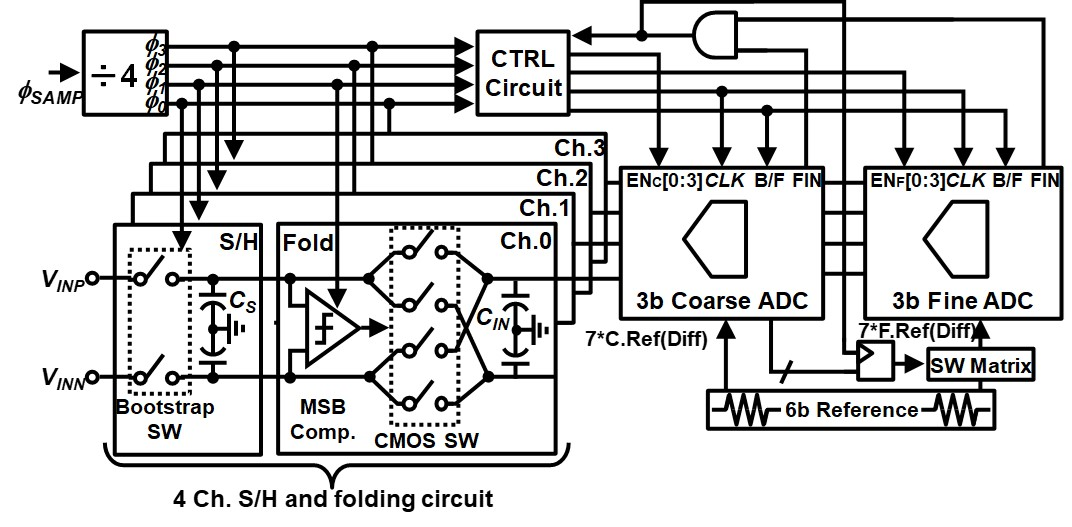
\includegraphics[width=1\textwidth]{figure/chap3/fig7.jpg}
  \caption{Block diagram of the 7-bit subranging ADC. DAFS is applied to the 3-bit coarse and fine sub-ADCs.}
  \label{fig-3-7}
\end{figure}

The 7-bit subranging ADC's block diagram is shown in Fig.\ref{fig-3-7}. An MSB (1-bit) is gained in the folding circuit, and 3-bits are acquired from each of the coarse and fine sub-ADCs. All results are added together to generate the 7-bit output. By using four times interleaved S/H and folding circuits, a four phase pipeline operation is realized to enhance the subranging ADC throughput and enable DAFS operation described in Section 3.2 (this will be explained later on). Folding circuits are capable of not only a low power MSB decision; they also halve the fine ADC reference (Fine ref.) transition. Since the fine ref. settling requirement is greatly relaxed, the settling can be completed within the ADC reset time and the subranging ADC does not require additional reset phases. Lastly, we should note that the coarse and fine sub-ADCs are a single channel and not time-interleaved. At each phase, the sub-ADCs switches the input and configures the channel to convert. 

\begin{figure}
\centering
  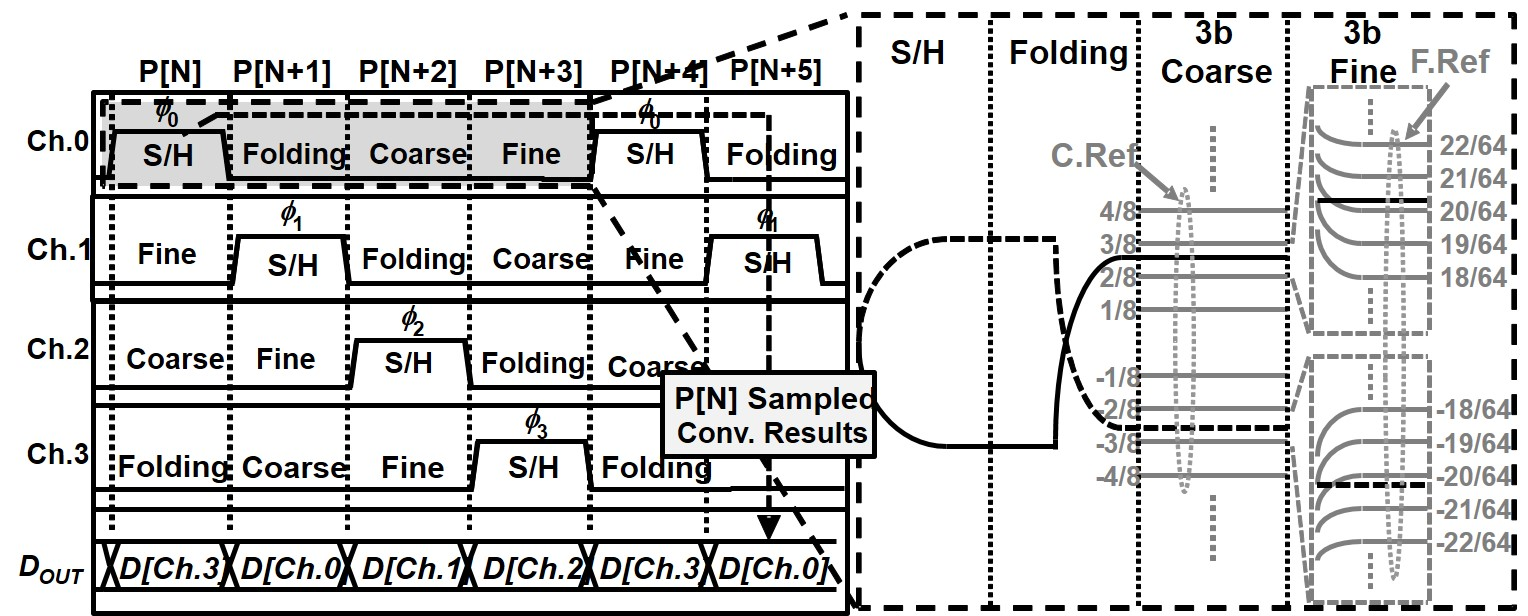
\includegraphics[width=1\textwidth]{figure/chap3/fig8.jpg}
  \caption{Block diagram of the 7-bit subranging ADC. DAFS is applied to the 3-bit coarse and fine sub-ADCs.}
  \label{fig-3-8}
\end{figure}

\begin{figure}
\centering
  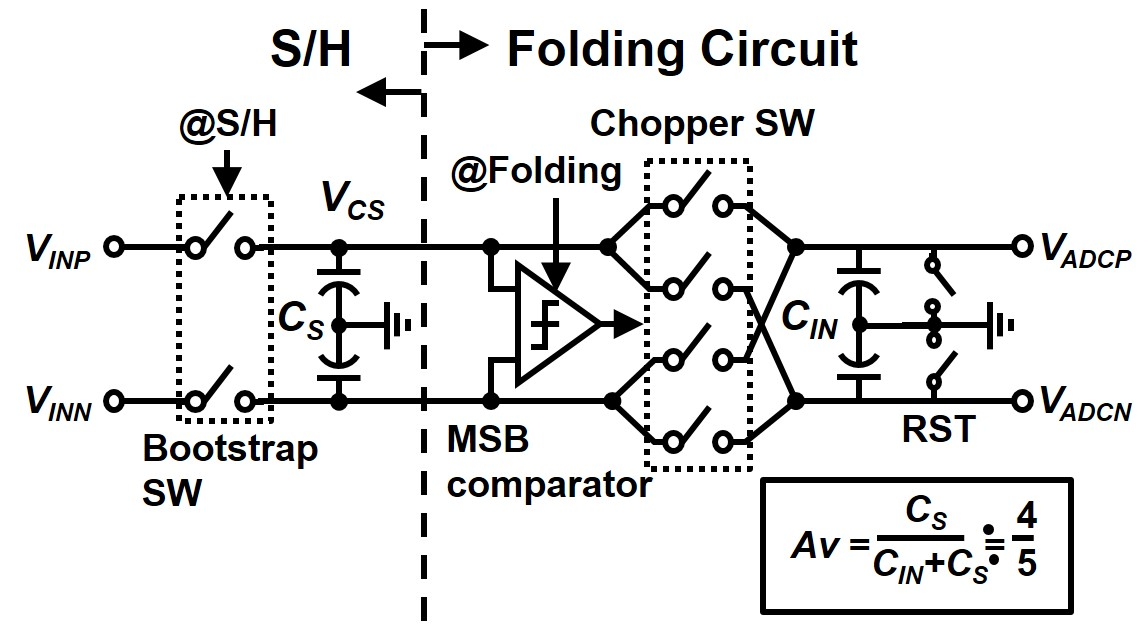
\includegraphics[width=1\textwidth]{figure/chap3/fig9a.jpg}
  %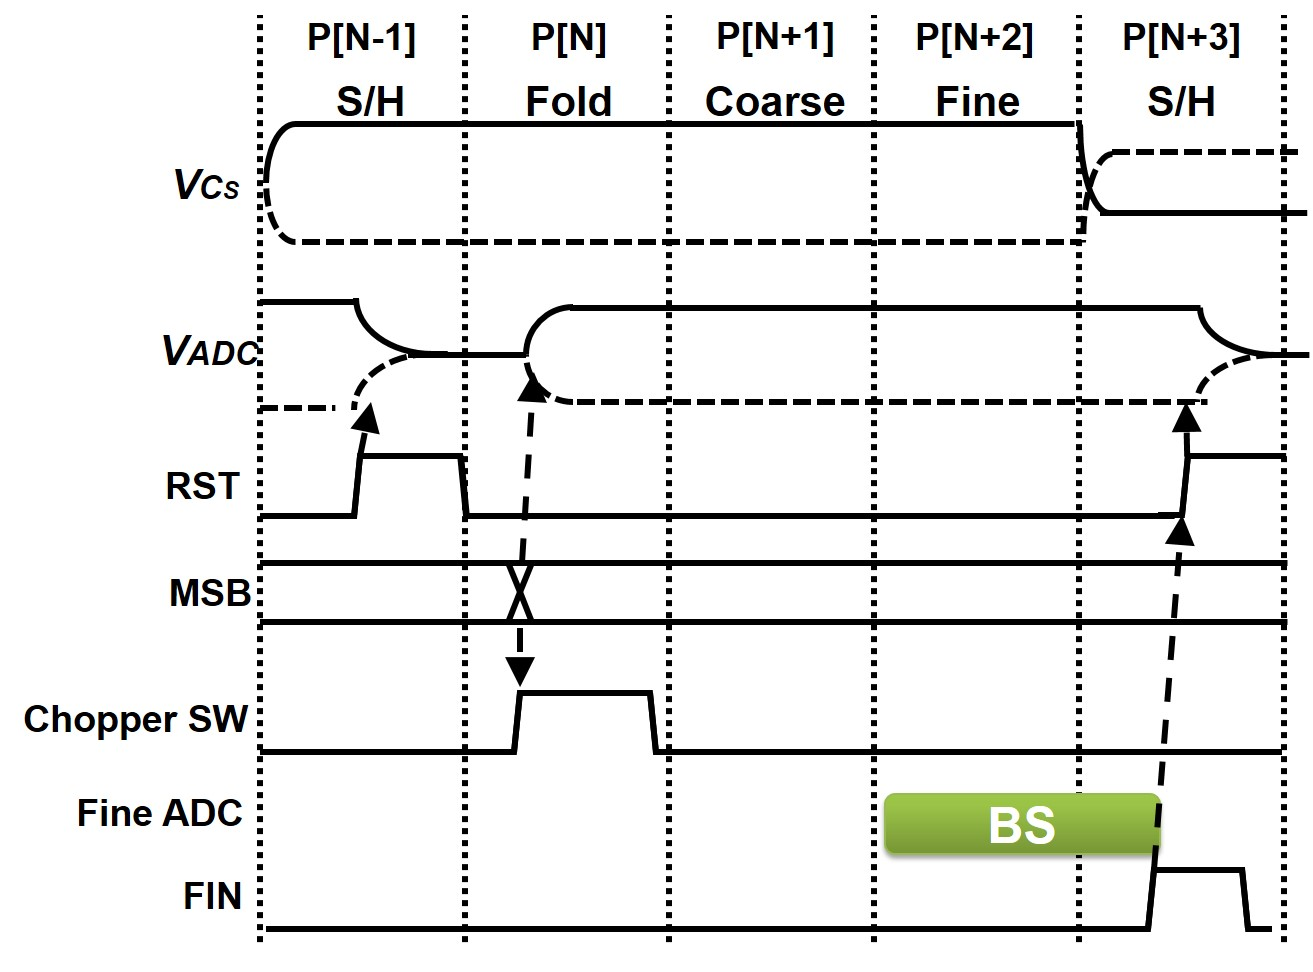
\includegraphics[width=1\textwidth]{figure/chap3/fig9b.jpg}
  \caption{Schematic of the full implementation of S/H and folding circuits.}
  \label{fig-3-9}
\end{figure}

The subranging ADC's conversion consists of four conversion phases: S/H, folding, coarse conversion, and fine conversion. Fig.\ref{fig-3-8} shows the operation of the four channels (Ch.0-3), and note that each channel operates with a conversion phase rotated 90 degrees. The ADC conversion is explained by focusing on the operation of Ch.0 as an example. Here, we will assume that at a certain phase P[N], Ch.0 performs S/H. The sampling switch is closed and the input signal (\textit{V${}_{IN}$}) is sampled to capacitor \textit{C${}_{S}$}, and the switch opens at the end of P[N]. At P[N+1], the MSB comparator of the folding circuit is activated and decides the MSB and simultaneously, the MSB comparator results are used to switch the chopper circuit, which rectifies \textit{V${}_{IN}$}. Next, at P[N+2], the 3-bit coarse conversion is performed. In this example, the input is somewhere between 2/8 and 3/8, so the seven fine refs. are switched depending on the results, like 17/64, 18/64, 19/64, etc. Finally, at P[N+3], 3-bit fine conversion \textit{zooms} the coarse converted range.

\subsection{S/H and Folding Circuits}

A specific schematic and timing chart of the S/H and folding circuits are shown in Fig.\ref{fig-3-9}. The folding circuit design is based on ref.\cite{verbruggen20102}, and realized rectifying with chopper switches instead of power-hungry opamps. While this folding circuit is low power, the output voltage (\textit{V${}_{ADC}$}) is the capacitive dividing of \textit{C${}_{S}$} and \textit{C${}_{in}$} and has a limited gain of \textit{A${}_{v}$} $\mathrm{<}$ 1. Since we designed this circuit with \textit{C${}_{S}$} =600fF and \textit{C${}_{in}$} =150fF, the gain is:
    \begin{equation}
        A_v=\frac{C_S}{C_S+C_{IN}}\cong \frac{4}{5}
    \end{equation}
\textit{C${}_{in}$} is the sum of the 130fF MOM capacitor and the 20fF comparator input capacitance, which is sized to suppress the comparator kickback. In folding circuits that only rectifies the signal at the frontend, there are no critical issues such as gain mismatch with the backend. The non-ideal \textit{A${}_{v}$} just attenuates the signal level the backend ADC receives, and therefore, \textit{A${}_{v}$} = 0.8 is acceptable. 

%In order for the DAFS to operate accurately, the S/H circuits must supply the desired input to the sub-ADCs even though their conversion is prolonged for an entire cycle. Here, we will explain how the S/H and folding circuit operates when ADC conversion is prolonged. To get the idea of the DAFS in subranging ADCs, the simplified timing chart is written with sub-ADC operating architectures in Fig.10. Firstly, we would like to focus on the Ch.2's coarse binary search conversion at P[N]. Since the conversion is prolonged until P[N+1], the same ADC input should be available at P[N+1] as well. In this case, this would not be a problem because the Ch.2's S/H phase does not appear until P[N+2]. However, problems would arise if the Ch.3's fine conversion, run at P[N+2], prolong until the S/H phase at P[N+3]. If \textit{V${}_{ADC}$} is reset before the A/D conversion is done, the results may be corrupted. 

%To counter this issue, the circuit has been designed so that \textit{V${}_{ADC}$} will not be reset until the fine sub-ADC finishes its conversion. Fig.9 (b) shows the timing chart of Ch.3 operation during P[N-1] to P[N+3]. As explained previously, the sampling switch is closed at S/H phase (P[N-1]) and \textit{V${}_{in}$} is charged to capacitor \textit{C${}_{S}$}. Meanwhile, the charge stored in the capacitor of folding circuit \textit{C${}_{in}$} is reset to \textit{V${}_{CM}$} by closing the RST switches. After S/H ends and folding phase (P[N]) starts, the MSB comparator is activated and configures the chopper switches. The chopper switches are only closed during the folding phase and the switches are kept open during coarse and fine conversions. Therefore, the voltage of the sampling capacitor (\textit{V${}_{CS}$}) transitions does not affect \textit{V${}_{ADC}$}. Although the fine conversion prolongs to P[N+3] and S/H are done, \textit{V${}_{ADC}$} is kept constant as long as the RST switches are open. In our design, the RST switches are triggered by the finish signal of the fine conversion itself to prevent the conversion from corrupting. We must mind that in the worst case, where the fine conversion is prolonged for the entire P[N+3], the charge in \textit{C${}_{in}$} can be barely reset. While this incomplete reset can leave some memory effect to the ADC input, the effect is suppressed by the ratio of \textit{C${}_{S}$} and \textit{C${}_{in}$}. Moreover, this incomplete reset occurs only when \textit{fs} is close to $fs{}_{maxFL}$ and the sub-ADC operates by binary search. Since the BF ratio can be as high as 0.98 in such high-speeds, the memory effect can happen only once in fifty conversions. By Matlab modeling, we confirmed that this effect will not harm the overall ADC resolution. 

\subsection{Live configuring with excess-delay accumulation}

\begin{figure}
\centering
  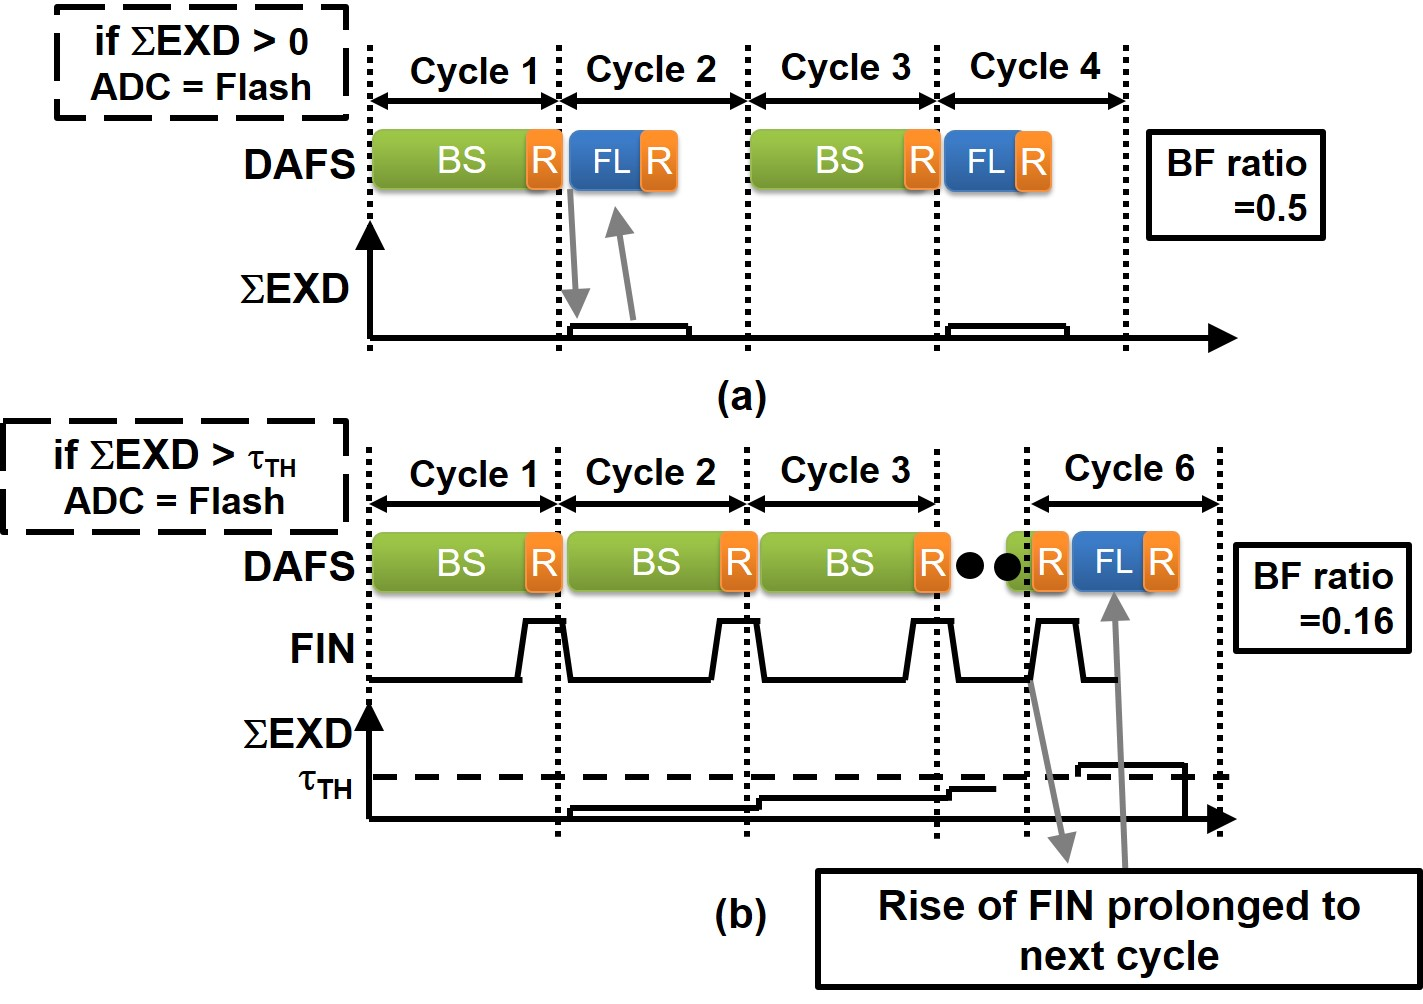
\includegraphics[width=1\textwidth]{figure/chap3/fig11.jpg}
  \caption{(a) DAFS operation without $\tau_{TH}$. Lowest BF ratio will be 0.5 since
flash operation will be inserted as soon as any EXD is detected. (b) DAFS operation with $\tau_{TH}$. ADC does not switch to flash until exceeds $\Sigma$ EXD.}
  \label{fig-3-11}
\end{figure}

Here, we describe the control circuit which configures the flash operation adaptively by detecting EXD. Since EXD is monitored in real-time, we will refer to the EXD monitoring and architecture controlling circuit as a \textit{live} configuring circuit from now on. The simplest live configuring can be implemented by seeing if the edge of the ADC reset phase continues into the next cycle or not, and if there is any EXD, the ADC architecture is switched to flash in the next cycle. However, this live configuring method has a critical weakness in that, the flash operation starts even if the detected EXD is very small. Fig.\ref{fig-3-11} (a) illustrates this issue, even with \textit{fs} slightly exceeding $fs{}_{maxBS}$ the flash operation begins in cycle 2. This is undesirable because the lower limit of the BF ratio will be as high as 0.5 and there will be a large power penalty.

\begin{figure}
\centering
  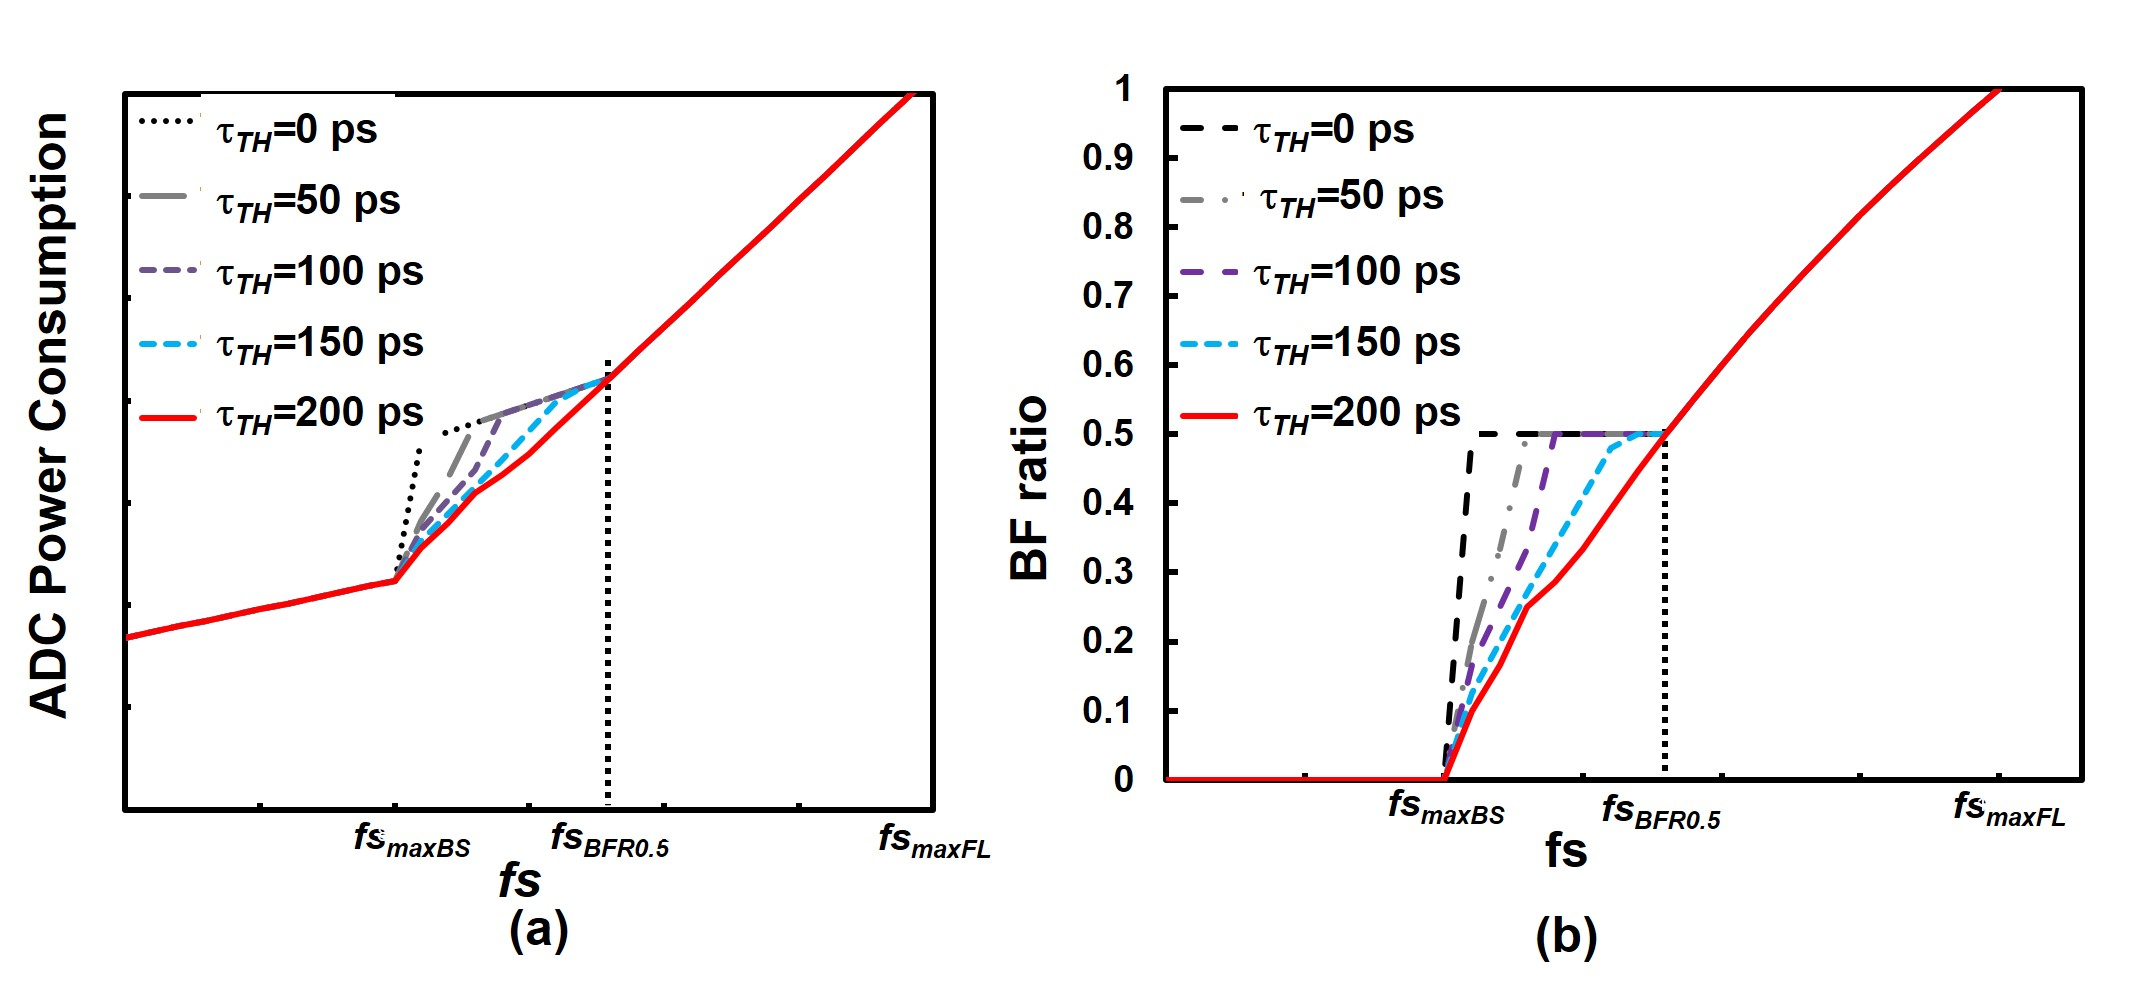
\includegraphics[width=1\textwidth]{figure/chap3/fig12.jpg}
  \caption{ (a) Power scaling with several values of $\tau_{TH}$. (b) versus BF ratio with several values of $\tau_{TH}$.}
  \label{fig-3-12}
\end{figure}

To lower the power consumption, the number of flash operations should be minimized. To realize this, live configuring with excess-delay accumulation is proposed. The timing chart for such a technique is shown in Fig.\ref{fig-3-11} (b). Here, even though a limited amount of EXD is produced in cycle 1, the flash operation does not start until the accumulated excess-delay ($\Sigma{\mathrm{EXD}}$) exceeds the threshold \textit{$\tau_{TH}$}. Therefore, if the produced EXD is very small, the ADC operates a number of cycles until $\Sigma$ EXD is accumulated to a sufficient amount of \textit{$\tau_{TH}$}.  In this example, the ADC operates 5 cycles until the live configuring circuit switches the ADC to flash, which results in BF ratio of 0.16. The ideal value of \textit{$\tau_{TH}$} should be chosen to minimize the number of flash operations, which is true when the EXD subtracted by a single flash operation is smaller than the accumulated EXD ($\Sigma$EXD).
\begin{equation}
    {\tau }_{THideal} \mathrm{>}t_{cyc}-t_{FL} \label{eq3.18}
\end{equation}
From \eqref{eq3.18}, we can see that large value of \textit{$\tau _{TH}$} must be set to achieve good scaling for \textit{fs} near fs${}_{maxBS}$. However, it is challenging to install long timing thresholds because it can cause instability in the system easily. For practical implementation, we simply used the ideal \textit{$\tau _{TH}$} where \textit{t${}_{cyc}$} (1/\textit{fs}) is the value when BF ratio meets 0.5. Since the EXD produced by binary search and the EXD subtracted by flash are equal in this frequency ($t_{BS}-t_{CYC}=t_{CYC}-t_{FL}$), the ideal \textit{$\tau _{TH}$} of this frequency will be:
\begin{equation}
    {\tau }_{TH}=t_{BS}-t_{cyc}=\frac{t_{BS}-t_{FL}}{2} \label{eq3.19}
\end{equation}
By substituting values obtained from the simulation and calculating \eqref{eq3.19}, the value of \textit{$\tau_{TH}$}=200ps was obtained. In Fig.\ref{fig-3-12}, the power scaling and \textit{fs} versus BF ratio were plotted for several values of \textit{$\tau_{TH}$}, respectively. From Fig.\ref{fig-3-12} (b), we can tell that larger \textit{$\tau_{TH}$} becomes, the power scaling becomes closer to the ideal scaling during \textit{$fs_{maxBS}$} $\mathrm{<}$ \textit{fs} $\mathrm{<}$ \textit{$fs_{BFR0.5}$} and\textit{ $\tau_{TH}$} of 200ps is satisfactory.

Next, let us explain a gate level implementation of the live configuring circuit with threshold \textit{$\tau_{TH}$}. As discussed before, long timing thresholds can cause instability in the system but on the other hand, the power efficiency will worsen if the threshold is too small. Generating \textit{$\tau_{TH}$} in delay circuits also causes issues such as PVT drift, and calibration must be done to counter them. In our live configuring circuit, the threshold is implemented by using the rising edge of the reset (FIN) signal for EXD detection, instead of the falling edge. The FIN signal is a pulse that rises from the end of ADC conversion until completion of ADC reset (Fig.\ref{fig-3-4}); in other words, the live configuring circuit exploits the ADC reset time as a threshold \textit{$\tau_{TH}$}. Since the ADC reset time is around 150-250ps across PVT variations, sufficient ADC power scaling can be expected, according to Fig.\ref{fig-3-12}. 

\begin{figure}
\centering
  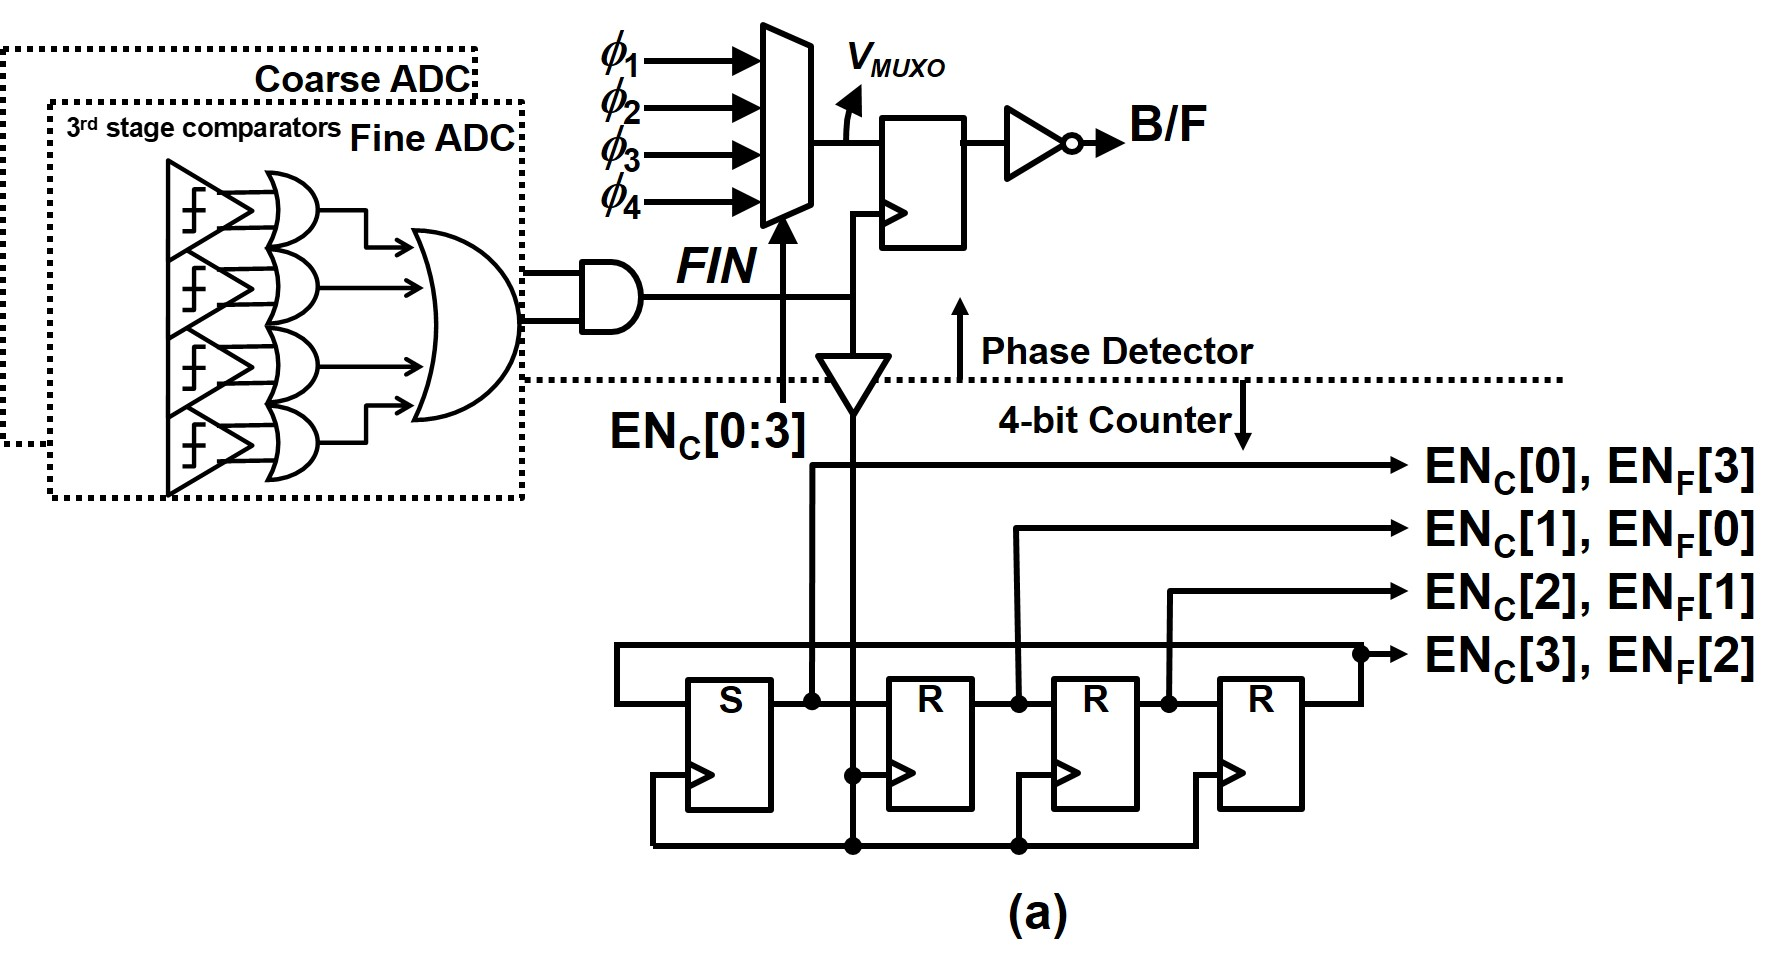
\includegraphics[width=1\textwidth]{figure/chap3/fig13a.jpg}
  %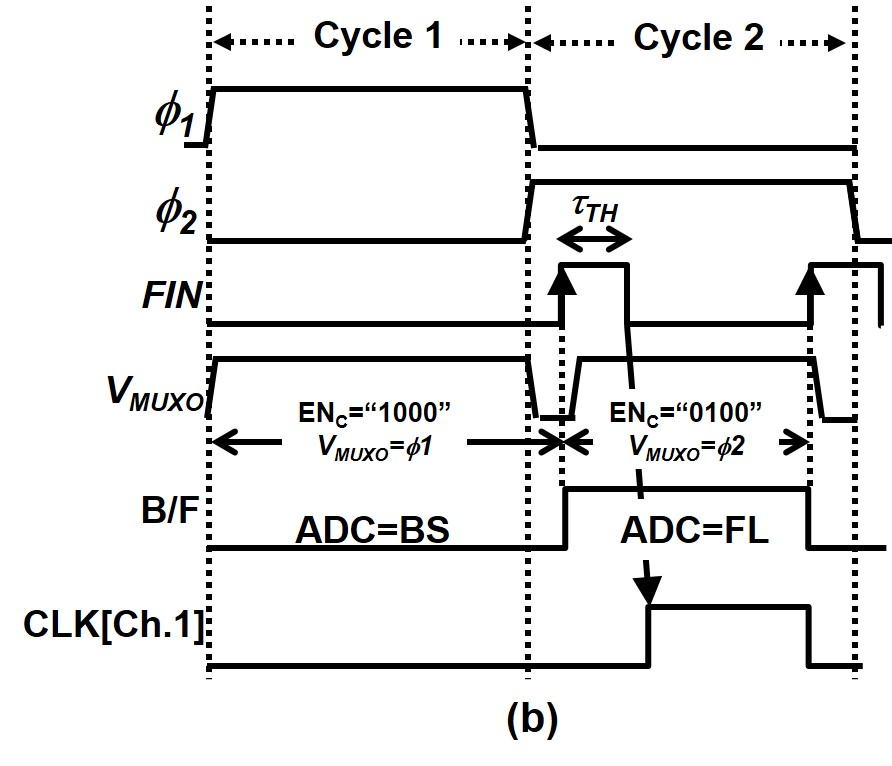
\includegraphics[width=0.6\textwidth]{figure/chap3/fig13b.jpg}
  \caption{ Schematic of the live configuring circuit which uses the pulse length of FIN as $\tau_{TH}$}
  \label{fig-3-13}
\end{figure}

A schematic and timing chart of the live configuring circuit is shown in Fig.\ref{fig-3-13}. The subranging ADC's coarse and fine sub-ADCs share the same B/F signal given from the live configuring circuit. Moreover, the FIN signal is generated by taking an AND of the FIN of both coarse and fine sub-ADCs. Therefore, the EXD monitoring is done based on the sub-ADC of a slower conversion, which is often the fine sub-ADC. By unifying the conversion finish signal, the complexity of the live configuring circuit can be greatly relaxed. The counter uses the rising edge of FIN as a trigger and switches the MUX output (\textit{$V{}_{MUXO}$}) between \textit{$\phi_{1-4}$}, which are 1/4 decimation of the sampling clock respectively. 

\subsection{Metastability issues}
The live configuring circuit in Fig.\ref{fig-3-13} may cause metastability in the flip-flop which generates the B/F signal. While this design did not cover the metastability issues, we here will discuss how its effect can be minimized.
The largest problem will occur when due to the flip-flop metastability, the B/F signal flips while the DAFS ADC is performing the conversion. 

Let's think of a transition when the B/F signal turns to BS to Flash during conversion. 
We notice that this will not cause any issues because since the comparators are activated successively, just configuring them to operate them at once will not corrupt the conversion results.
However, if the signal flips from Flash to BS will be a problem because we do not know which comparators were successively activated. Moreover, the BS ADC encodes the output noting that only one comparators are activated per MSB. Therefore, the B/F signal generation should be configured so that if there are signs of metastability, the signal should be close to BS. This can be achieved by making the NMOS size larger in the buffering inverter. 

\color{black}

%For example, in Fig.\ref{fig-3-13} (b), since the binary search conversion in cycle 1 is slow, the rising edge of\textit{FIN} does not appear until cycle 2. In this case, the live configuring circuit should change the ADC architecture to flash for the next cycle. 

%The multiplexer has a selector signal (EN${}_{C}$) of `1000` and outputs\textit{$\phi$1 }until the rising edge of FIN. Therefore, since \textit{$\phi$ 1} sets down at cycle 2, the DFF based phase detector (PD) latches \textit{$V{}_{MUXO}$} =0 at the FIN's rising edge. Since this latched result is inverted and used directly as the B/F signal, the ADC is reconfigured to operate as flash in cycle 2. Then, the delayed\textit{ }FIN signal triggers the counter circuit and EN${}_{C}$ is configured to `0100`, and therefore output of \textit{$V{}_{MUXO}$} will be \textit{$\phi$ 2}. After the conversion at cycle 2, FIN signal rises within the cycle and \textit{$V{}_{MUXO}$} =1 is latched by PD. For that reason, the ADC operation returns to binary search in cycle 3. Note that even though the FIN pulse is prolonged until cycle 3, because of the threshold \textit{$\phi_{TH}$},\textit{${}_{\ }$}the live configuring circuit ignores this event. By adding the live configuring circuit to the ADC, the DFF transition and inverter delay are added to its critical path, and worsens the ADC's $fs{}_{max}$ about 10\%. 

%Not only the counter outputs (EN${}_{C}$ and EN${}_{F}$) are used to control the MUX, but the signals are also used to determine which channel the sub-ADC converts. EN${}_{C}$ and EN${}_{F}$ are provided to the coarse and fine sub-ADCs respectively, as shown in Fig.13. The same signals are used for EN${}_{C}$ and EN${}_{F}$ and only the bit assignment differs. The sub-ADC operation with EN${}_{C}$, EN${}_{F}$ signals are shown in Fig.10. For example, at P[N], EN${}_{C}$ is `0010` and the coarse sub-ADC uses the third channel (Ch.2) as the input.

\subsection{Sub-ADC designs}

\begin{figure}
\centering
  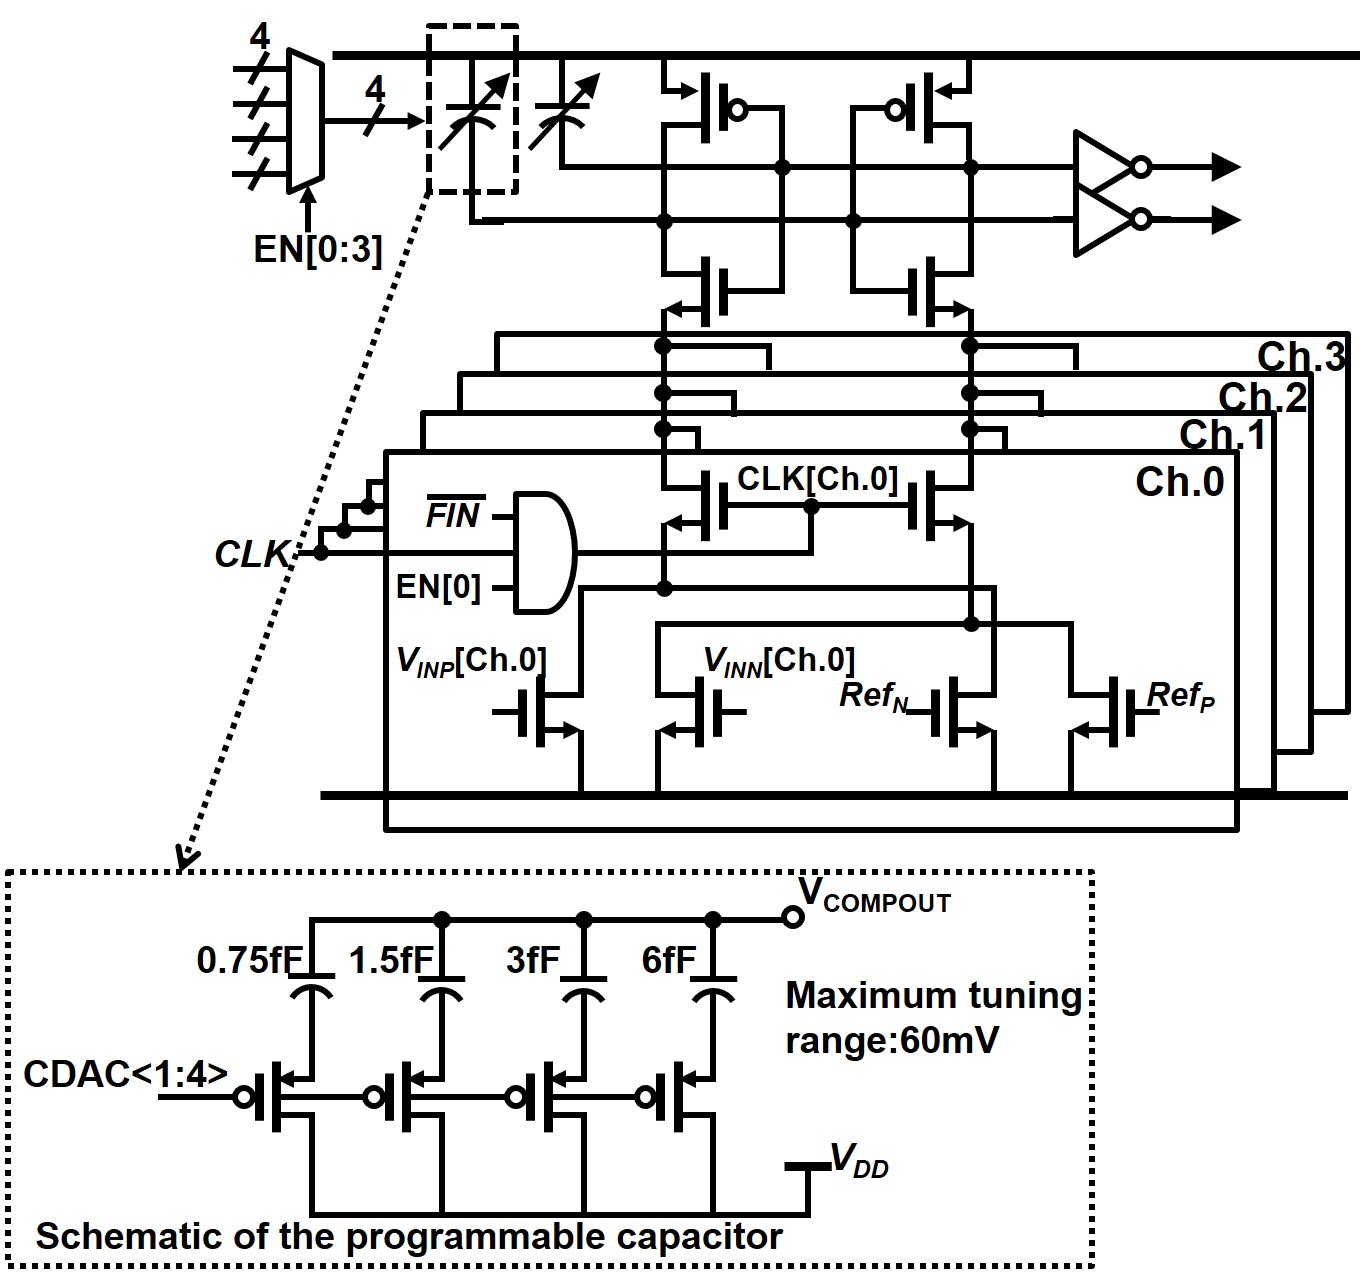
\includegraphics[width=0.8\textwidth]{figure/chap3/fig14.jpg}
  %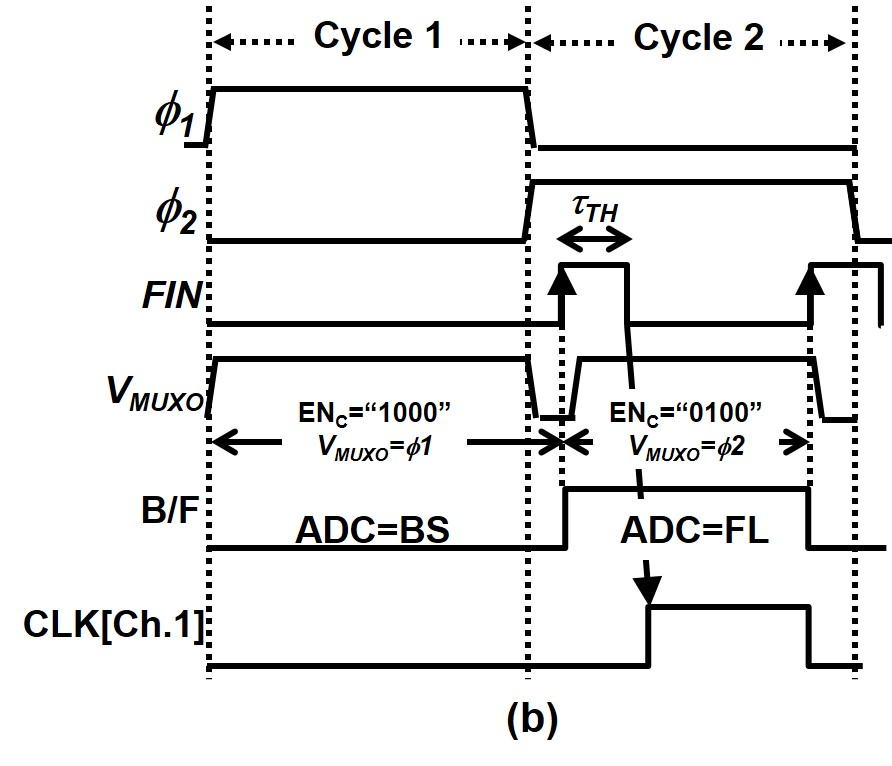
\includegraphics[width=0.6\textwidth]{figure/chap3/fig13b.jpg}
  \caption{Schematic of the comparator with four channel input. The input channel is determined by signal EN[0:3]. The programmable load capacitance used for offset compensation is shown as well.}
  \label{fig-3-14}
\end{figure}

Now let us describe the binary search/flash reconfigurable ADC used in the sub-ADC. While the comparator mismatch requirements can be relaxed by having redundant bits in the 3-bit sub-ADCs, there are expenses of increased power and area. For example, the calibration procedure can be reduced 60\% by implementing the sub-ADC with the redundancy of 3.5-bit, but the power and area increase 60\%, respectively. We chose to implement the 3-bit sub-ADC without redundancy to minimize power consumption and area and compensate for the comparator mismatch by foreground calibration, which is described later on. Fig.\ref{fig-3-14} shows the schematic of the comparator, based on ref.\cite{proesel20108}, which is used in the sub-ADC. Note that the reset transistors are omitted for simplicity. The comparator is clocked, and it has four input transistors for the differential \textit{V${}_{IN}$} and reference. 

To compensate with the four channel S/H, this comparator has multiple input transistor pairs each corresponding to the respective channels. Fig.\ref{fig-3-14} shows the input transistors for Ch.0 and the activation circuit made of 3-input AND. As in Fig.10, the Ch.0 comparator input pairs are activated when EN[0] is \textit{High}. Multi-input comparators can be implemented by configuring \textit{V${}_{IN}$} with switches every cycle, but in such cases, \textit{V${}_{IN}$} settling becomes a critical issue in GS/s operations and an additional settling phase will be required. While the multiple input transistor pair approach is suited for high-speed operation, the mismatch generates different offset voltages between the input pairs and corrupts the ADC linearity. 

%Furthermore, while the two input comparators have a tipping-point near $\mathrm{\sim}$\textit{V${}_{CM}$}, the four input current summing comparators are built-in offset comparators and has a tipping-point at \textit{V${}_{CM}$} +\textit{REF}, where \textit{REF} is the applied offset. Since the input transistor's overdrive voltage (\textit{V${}_{OD}$}) at the tipping-point increases, the effect of the mismatch is also emphasized as well as $V_{OD} \times \Delta \beta$ and four input comparator suffer several times larger offset than two input comparators \cite{sumanen2002cmos}. Even though increasing the transistor size is an effective way to relax the offset \cite{pelgrom1989matching}, there are trade-offs between kickback, power, speed, and calibration complexity. In this design, the transistor size was decided based on Monte-Carlo simulation results to achieve GS/s and low power performance with the aid of calibration.

Lastly, the calibration methods are briefly explained. Since the offset between the multiple input transistor pairs must be nulled, the mapping codes to cancel the offset are acquired via foreground calibration for each channel. The mapping codes are digital values which configure the programmable capacitors. To suppress the comparator offset to under LSB/2, the smallest calibration step of 3 mV was chosen, which ended up with a unit capacitor sizing of 0.75 fF. We chose to design a 4-bit capacitor bank to compensate with the comparator's 3 $\sigma$ mismatch of 60 mV. When the ADC is operating, the mapping codes are switched every cycle to cancel the varying offsets. The comparator's foreground calibration can be done simply since reference voltages are supplied via the on-chip R-DAC. By shorting the comparator input with the reference voltage, a binary search can be conducted by switching the load capacitances as described in ref.\cite{yoshioka20158}. After the binary search, mapping code which cancels the offset is obtained, and these codes will be saved for each input pairs of Ch.0-3 since each of them has different offsets. As the ADC operates, these mapped codes are switched every cycle by the MUX.

\section{Results and Discussion}

\subsection{Measured Results}

\begin{figure}
\centering
  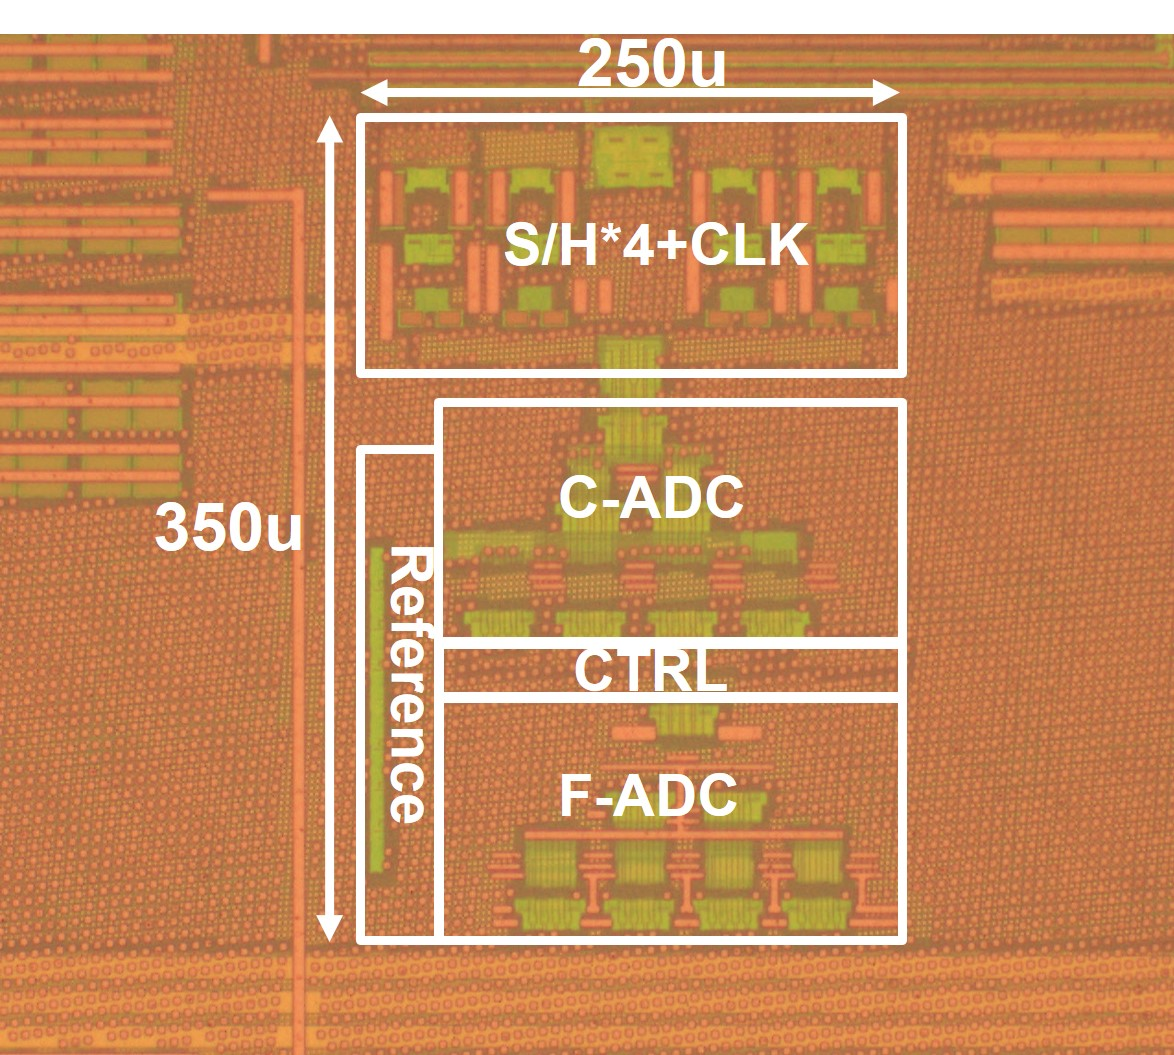
\includegraphics[width=0.7\textwidth]{figure/chap3/fig15.jpg}
  \caption{Chip micrograph.}
  \label{fig-3-15}
\end{figure}
\begin{figure}
\centering
  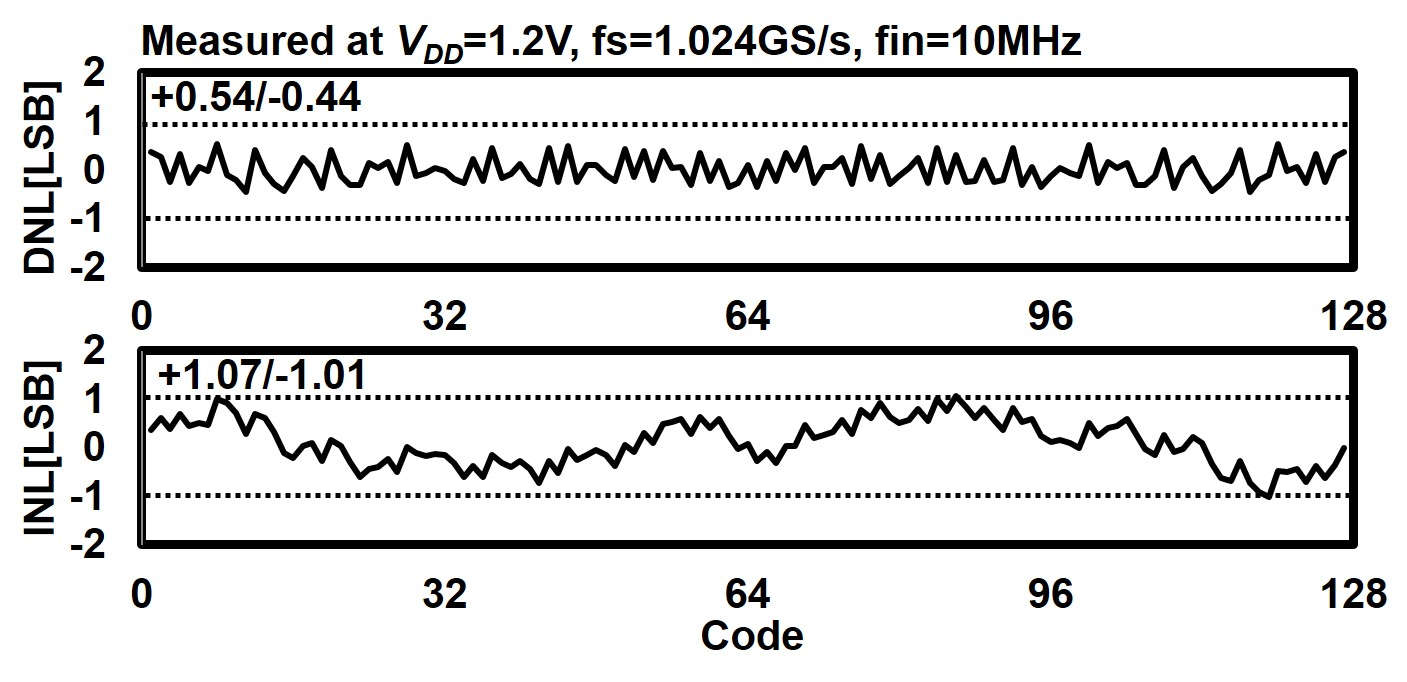
\includegraphics[width=1\textwidth]{figure/chap3/fig16.jpg}
  \caption{Measured DNL/INL after foreground comparator offset calibration}
  \label{fig-3-16}
\end{figure}


The subranging ADC with DAFS was implemented in 65nm CMOS process. Fig.\ref{fig-3-15} shows the chip micrograph, and the ADC occupied an area of 250 x 350 um. A foreground calibration was done to cancel the comparator offsets. On the other hand, no tuning was applied to the live configuring circuits since they can tolerate PVT variations. Fig.\ref{fig-3-16} plots DNL/INL after calibration, respectively measured at \textit{fs}=1024 MS/s and \textit{fin}=10 MHz. Besides, we did not observe any difference in the linearity when the sub-ADC architecture was switched between flash and binary search.

%Even with the calibration, the INL did not settle within $<$ 1 LSB. The comparator mismatch cannot be fully canceled because the common-mode of the fine sub-ADC reference changes greatly depending on the coarse conversion results. Since this produces additional common-mode triggered offsets, the R-DAC top and bottom voltages were reduced to 0.85 V and 0.35 V, respectively. Even though narrowing the fullscale does not cause noise problems in this design, it may be problematic in ADCs with higher resolutions. The reference common-mode can be stabilized by employing C-DACs in subranging ADCs \cite{asada20096bit}, with an overhead of C-DAC area and a finite settling time. 

\begin{figure}
\centering
  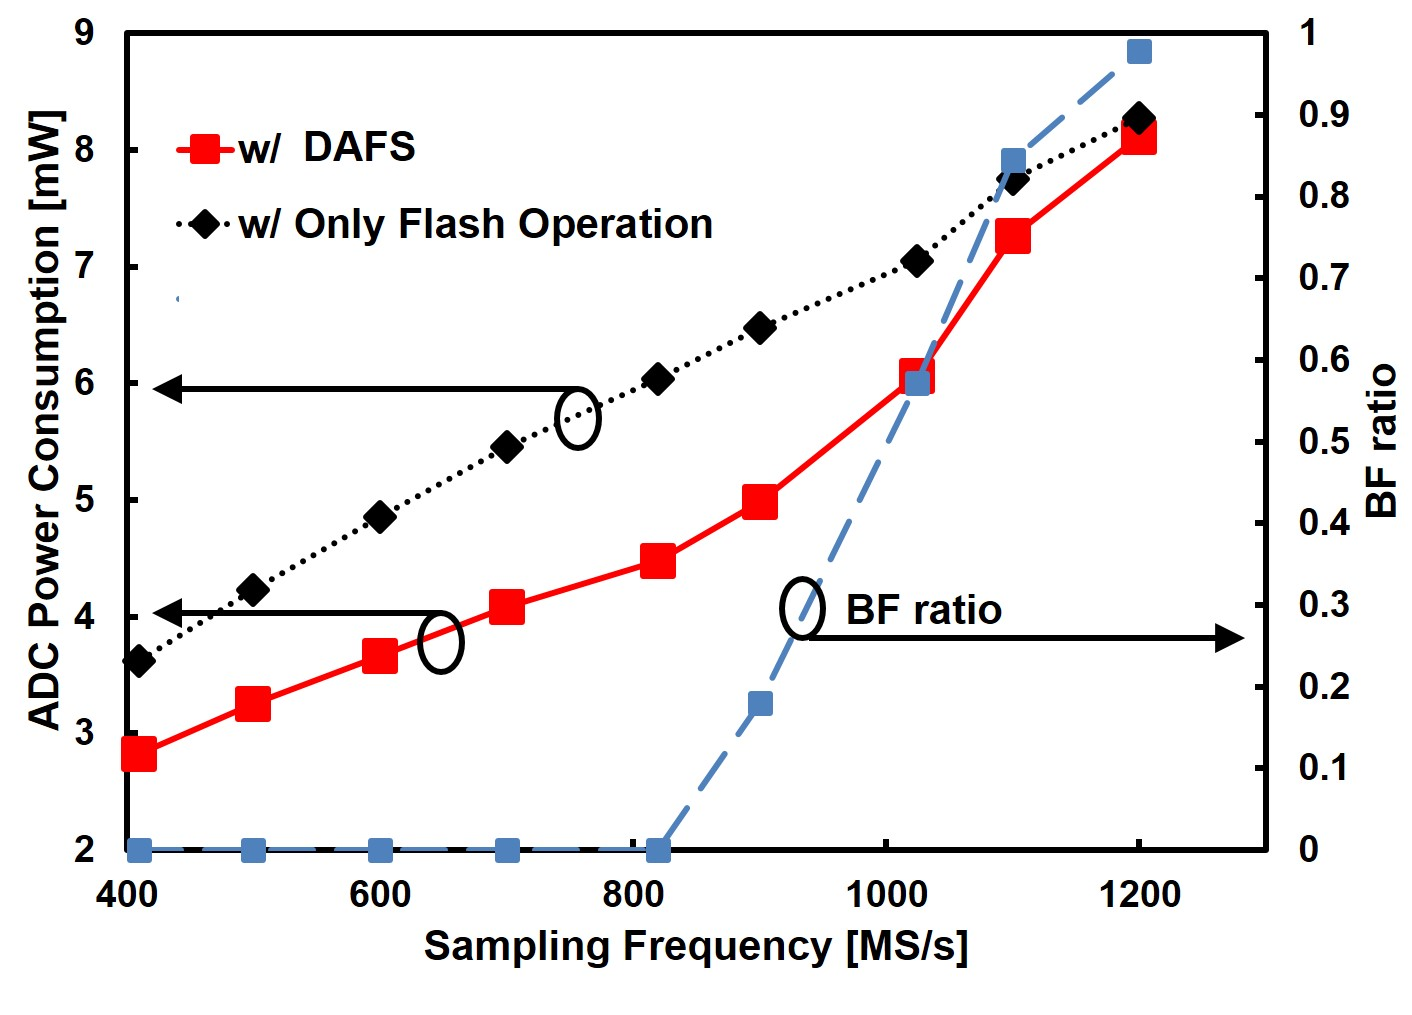
\includegraphics[width=0.9\textwidth]{figure/chap3/fig17.jpg}
  \caption{Measured power scaling of the subranging ADC, with and without
DAFS. The BF ratio was measured and plotted as well.}
  \label{fig-3-17}
\end{figure}

The measured power scaling characteristic of the subranging ADC is shown in Fig.\ref{fig-3-17}. The sub-ADCs are programmable to operate either as DAFS or flash only, and the power scaling for both operation modes are shown. While the power scaling is linear when sub-ADCs operate only with flash, superlinear power scaling was observed with DAFS during high-speed operation at 820 MS/s to 1220 MS/s. The BF ratio was measured by acquiring the architecture configuring signal (B/F) and is plotted as well. Beyond 820 MS/s ($fs_{maxBS}$), the live configuring circuit detected EXD and began to insert flash operations. As \textit{fs} increased, more flash operations were inserted and made the power scaling superlinear. At 1220 MS/s ($fs_{maxFL}$), the power consumption reached nearly that of flash only operation and the BF ratio reached 0.98. Similar power scaling characteristics were confirmed in all ten measured samples, which show the robustness of the live configuring. A peak FoM of 85 fJ/conv. was obtained at $fs_{maxBS}$: 820 MS/s. DAFS achieves a 30\% power reduction compared with the power consumed by sub-ADCs operating only with flash. However, this result is smaller than what we expected in Section 3.2. This result will be analyzed later on.

\begin{figure}
\centering
  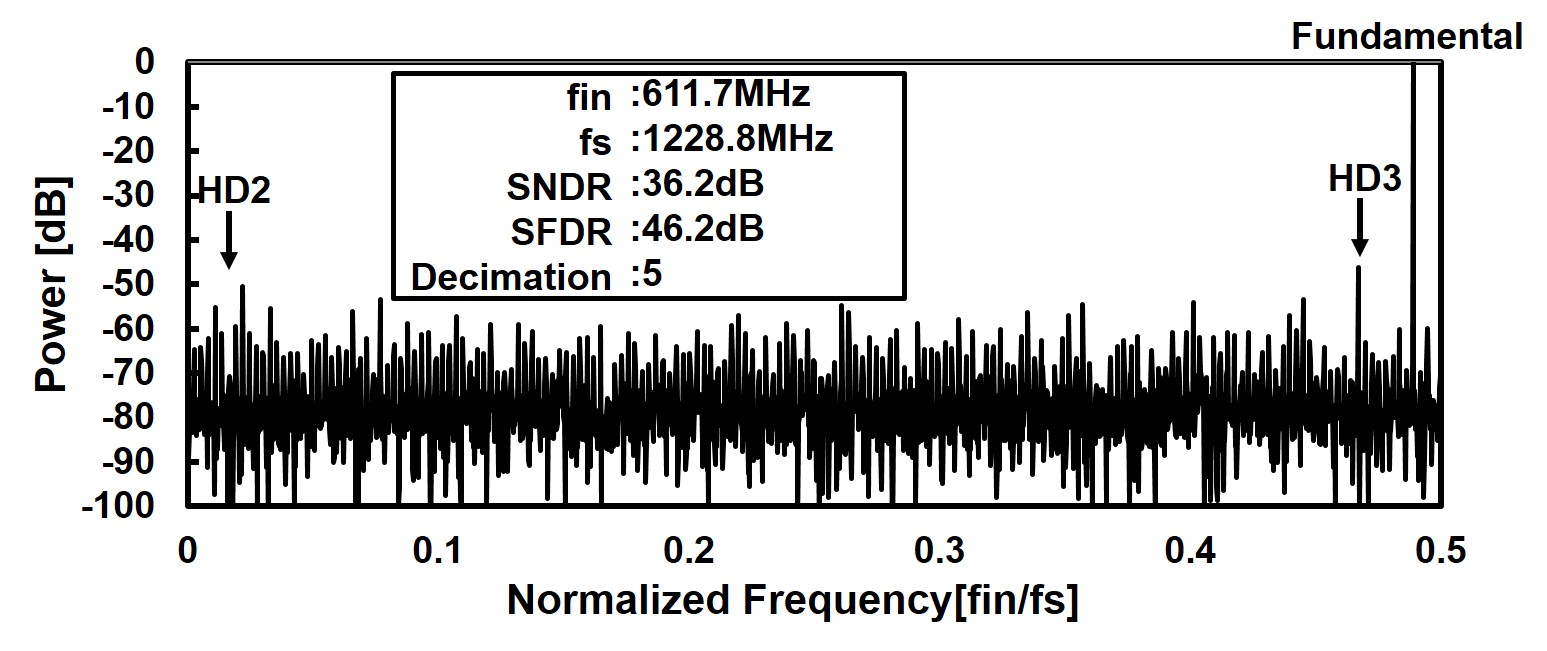
\includegraphics[width=0.9\textwidth]{figure/chap3/fig18.jpg}
  \caption{Measured 4096-point FFT spectrum at the written condition.}
  \label{fig-3-18}
\end{figure}
\begin{figure}
\centering
  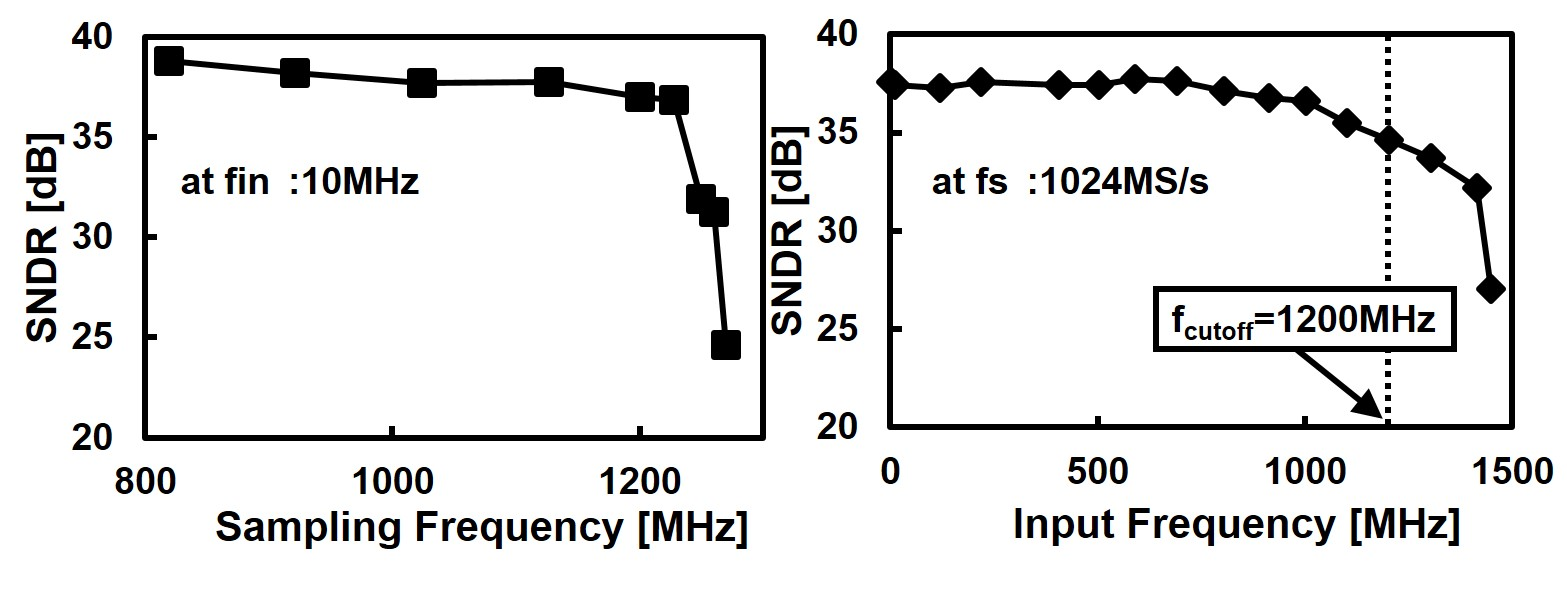
\includegraphics[width=0.9\textwidth]{figure/chap3/fig19.jpg}
  \caption{(a) Measured versus SNDR. (b) Measured versus SNDR}
  \label{fig-3-19}
\end{figure}

The 4096 FFT spectrum measured at 1220MS/s is plotted in Fig.\ref{fig-3-18}, and \textit{fs} and \textit{fin} versus SNDR is plotted in Fig.\ref{fig-3-19}. The nonlinearity of the ADC was mostly due to comparator offsets, while the gain mismatch and timing-skew did not impact the ADC resolution. In Fig.\ref{fig-3-19} (a), there was a brick wall at 1250MS/s where SNDR suddenly deteriorated. This happens because \textit{fs} exceeded $fs_{maxFL}$, the coarse sub-ADC started to make conversion errors. In such cases, fine conversions become meaningless and the resolution greatly degrades.  

\subsection{Discussions}

\begin{figure}
\centering
  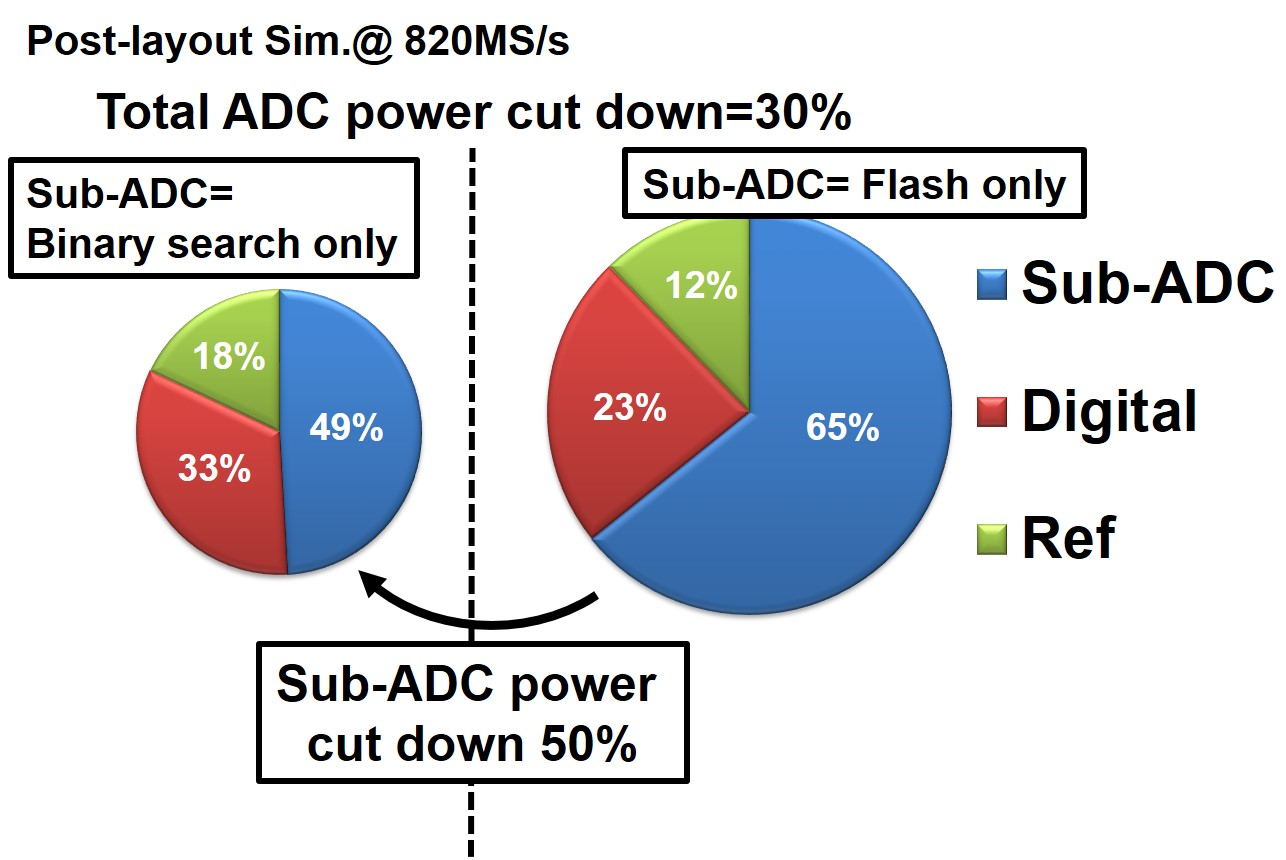
\includegraphics[width=0.9\textwidth]{figure/chap3/fig20.jpg}
  \caption{Power breakdown of the ADC at 820 MS/s with sub-ADC operated
only with binary search and flash respectively.}
  \label{fig-3-20}
\end{figure}

Fig.\ref{fig-3-20} shows the power breakdown of the ADC acquired from the post-layout simulation at 820 MS/s. Two cases are shown, one in which the sub-ADC operates as only a binary search and one as a flash. If we focus on the sub-ADC power consumption, a 50\% power reduction is achieved by reconfiguring the ADC architectures, which is close to the predictions made in Section 3.2. However, since the power of the digital and reference circuits does not change with DAFS, these become the bottleneck when scaling the entire ADC power. If we extend the sub-ADC resolution to beyond 4-bits, the power consumption of sub-ADC will be dominant since \textit{$P_{FL}$} increases exponentially. Since the power of other circuits hardly changes, DAFS power scaling will be emphasized. However, aiming further ADC resolution will result in stricter timing-skew and gain mismatch requirements and more effort must be spared for sampling frontend designs.

\begin{figure}
\centering
  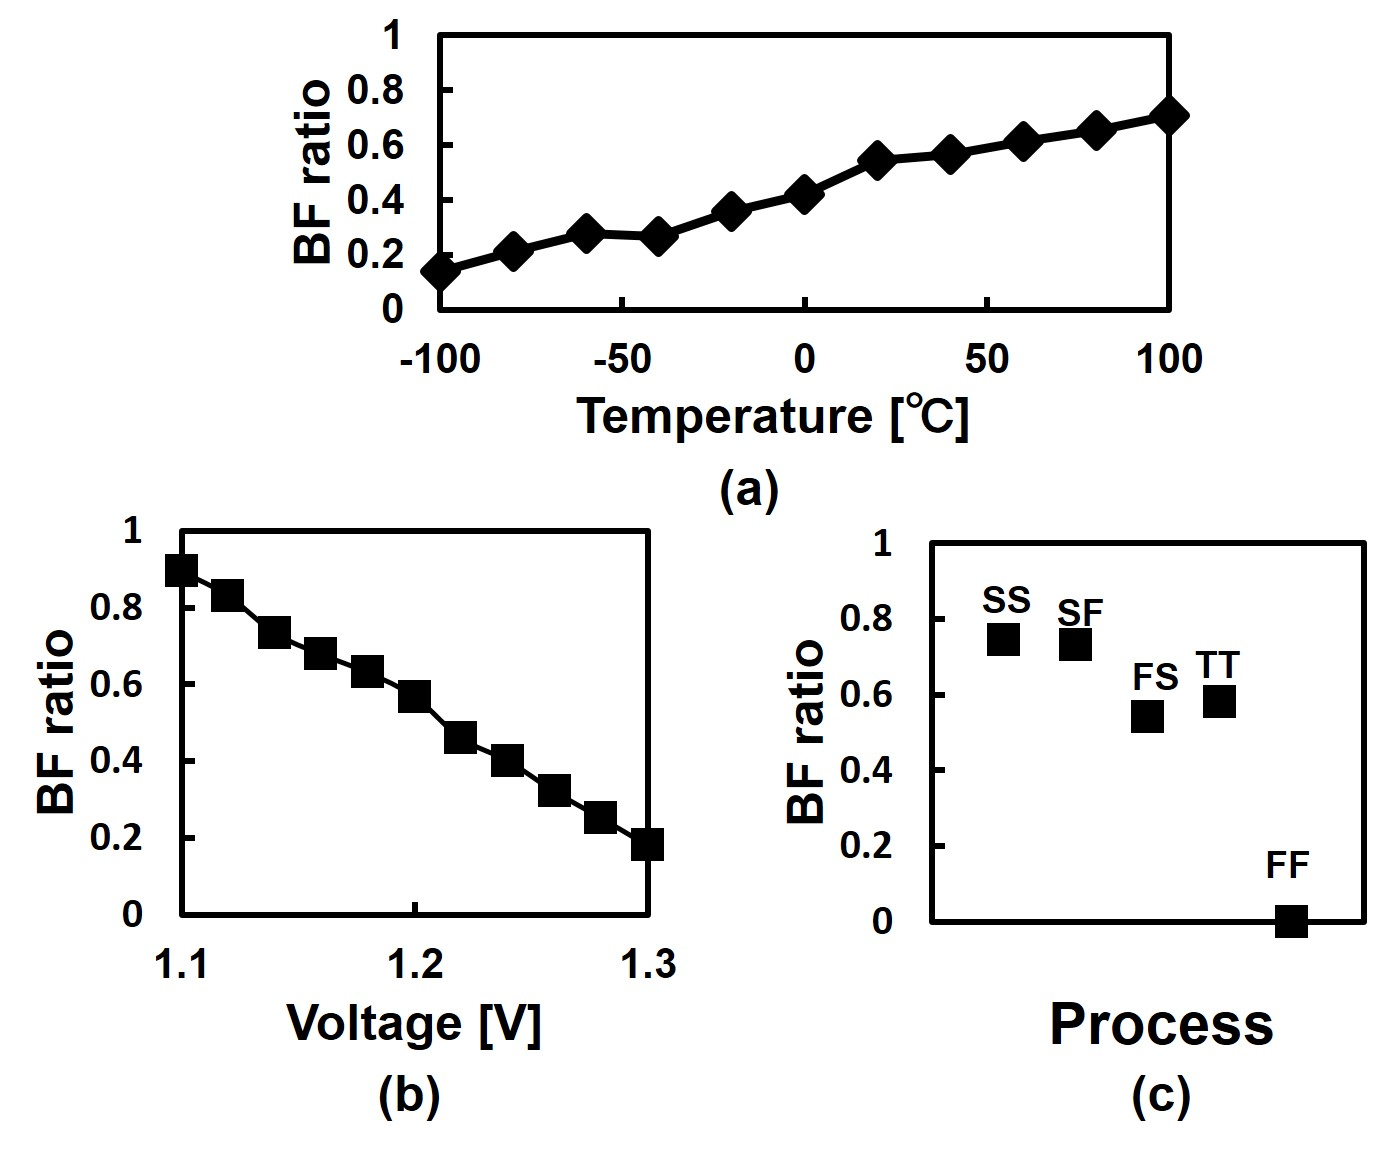
\includegraphics[width=0.9\textwidth]{figure/chap3/fig23.jpg}
  \caption{PVT variations versus BF ratio is shown. Interestingly, DAFS can operate to cancel out PVT variation effects, relaxing the speed margins of the high-speed ADC. (a) Temperature (b) Voltage (c) Process variations are plotted respectively.}
  \label{fig-3-21}
\end{figure}

In Fig.\ref{fig-3-21}, each PVT were varied in post-layout simulation, and the resulting change of BF ratio was observed at \textit{fs}=1GS/s. As expected, the BF ratio tracks the transistor speed shift due to the PVT variation. 
Since the speed of comparator based ADCs is sensitive to PVT, these characteristics greatly relax the design margin of the ADC.
Let's imagine a BS ADC designed to operate in 800 MS/s at the typical condition.
However, in the worst PVT cases, the maximum speed can degrade as low as 600 MS/s.
In such cases, the ADC can insert flash operations to extend its maximum speed in the expense of extra power consumptions. Note that this does not hurt the power efficiency of the typical conditions because it will operate fully as a BS ADC.
Compared with typical conditions, the sub-ADC power consumption was 20\% higher under SS conditions and 40\% lower under FF conditions in Fig.\ref{fig-3-21} (c).

\begin{table}
\centering
  \caption{Comparison with state-of-the-art high-speed ADCs.}
  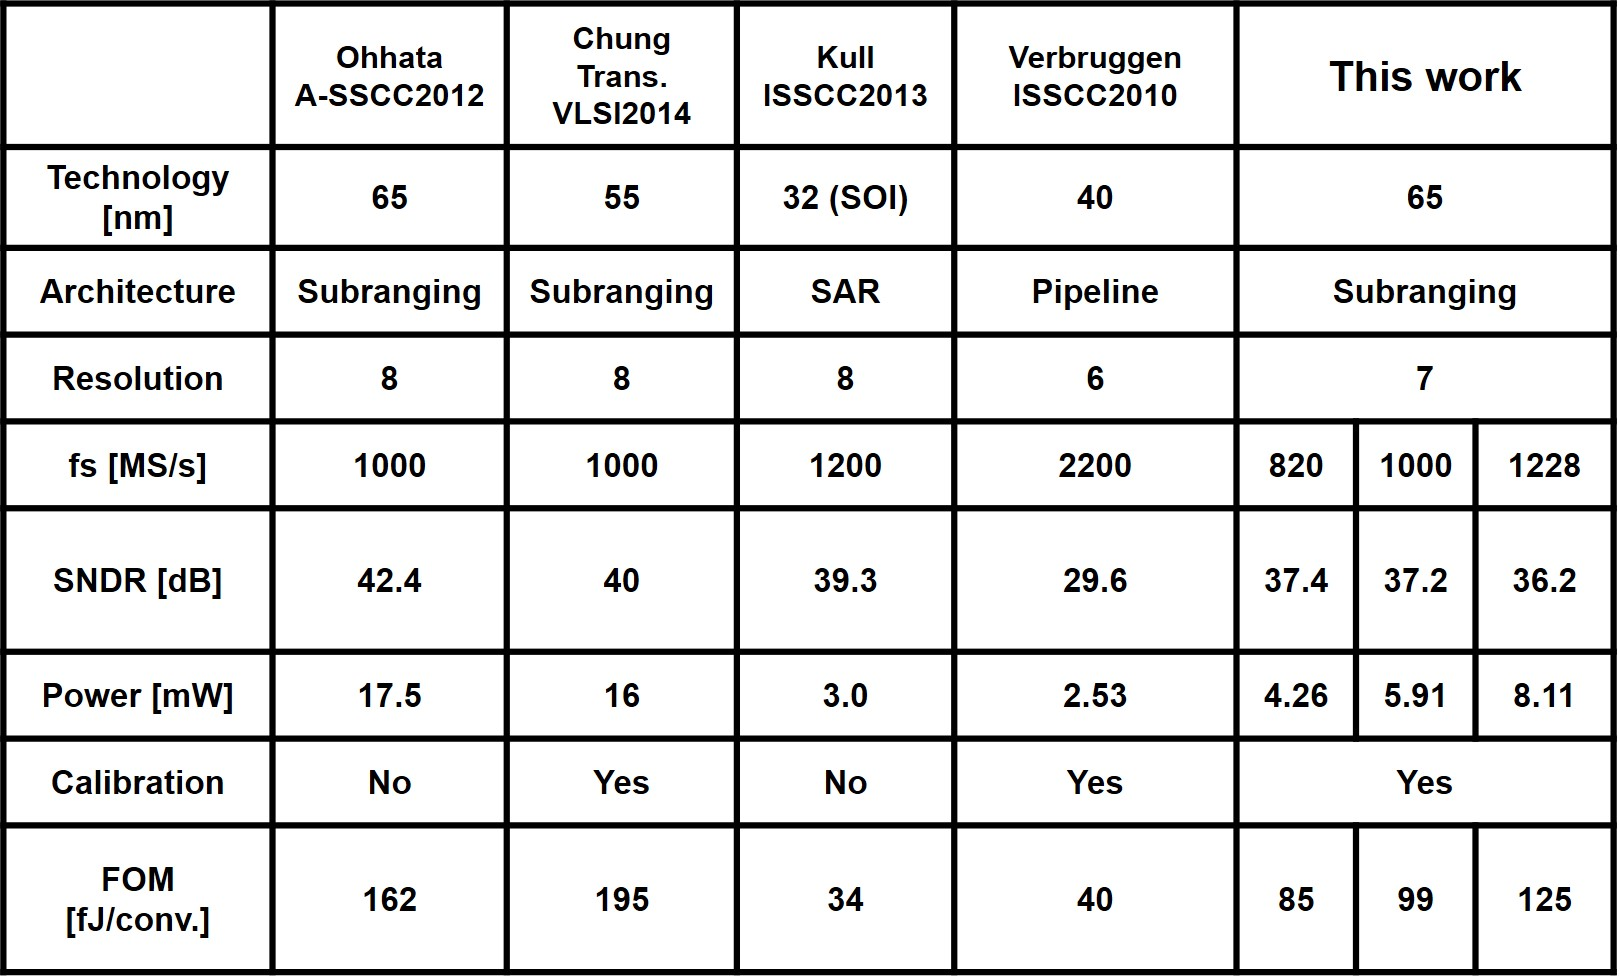
\includegraphics[width=1\textwidth]{figure/chap3/table1.jpg}
  
  \label{tab-3-1}
\end{table}

 Lastly, TABLE \ref{tab-3-1} compares our ADC with other state-of-the-art low resolution GS/s ADCs. Compared with conventional subranging ADCs, ours achieved two times better power efficiency. However, the SAR and pipeline ADCs of ref.\cite{verbruggen20102} and \cite{kullsar} have better power efficiencies. It is worth noting that the power consumption and speed of comparator based ADCs scale significantly with CMOS device scaling. When designed with more advanced CMOS devices, this ADC is expected to operate with a performance comparable to the references. Moreover, this ADC is the first to have superlinear power scaling with GS/s operation.

\section{Conclusions}

A subranging ADC with Dynamic Architecture and Frequency Scaling (DAFS) was presented. While operating at over 1GS/s, the ADC accomplishes superlinear power scaling by adaptively reconfiguring the sub-ADC architecture between binary search and flash. The architecture reconfiguration is done by monitoring the excess-delay of the conversion, and flash operation are used to cancel the excess-delay. DAFS not only improves the power scaling significantly but compensates for the transistor speed shift due to PVT variation which can be used to relax the design margin in high-speed ADCs.

A 7-bit subranging ADC was designed in 65nm CMOS in which the DAFS was applied to the sub-ADC. The DAFS operation was confirmed in the range of 820-1220MS/s, and achieving superlinear power scaling. When compared to the ADC performance with DAFS disabled, a maximum of 30\% power reduction was achieved. This subranging ADC achieved peak FoM of 85fJ/conv. at 820MS/s, which is nearly a twofold improvement over the conventional subranging ADCs.
